\documentclass[12pt]{article}
\usepackage[usenames, dvipsnames, table]{xcolor}
\usepackage[utf8]{inputenc}
\usepackage[T1]{fontenc}
\usepackage{lmodern}
\usepackage{amsmath}
\usepackage{amsfonts}
\usepackage{comment}
\usepackage{wrapfig}
\usepackage{booktabs}
\usepackage{tikz}
\usepackage{gnuplottex}
\usepackage{epstopdf}
\usepackage{marginnote}
\usepackage{float}
\usetikzlibrary{tikzmark}
\usepackage{graphicx}
\usepackage{cancel}
\usepackage{bm}
\usepackage{mathtools}
\usepackage{hyperref}

\DeclareMathOperator{\sech}{sech}
\DeclareMathOperator{\csch}{csch}
\DeclareMathOperator{\arcsec}{arcsec}
\DeclareMathOperator{\arccot}{arcCot}
\DeclareMathOperator{\arccsc}{arcCsc}
\DeclareMathOperator{\arccosh}{arcCosh}
\DeclareMathOperator{\arcsinh}{arcsinh}
\DeclareMathOperator{\arctanh}{arctanh}
\DeclareMathOperator{\arcsech}{arcsech}
\DeclareMathOperator{\arccsch}{arcCsch}
\DeclareMathOperator{\arccoth}{arcCoth} 

\newif\ifquoteopen
\catcode`\"=\active % lets you define `"` as a macro
\DeclareRobustCommand*{"}{%
   \ifquoteopen
     \quoteopenfalse ''%
   \else
     \quoteopentrue ``%
   \fi
}

\PassOptionsToPackage{table}{xcolor}

\usepackage{soul}

\newcommand{\hlc}[2]{%
  \colorbox{#1!50}{$\displaystyle#2$}}


\usepackage[a4paper,
            total={170mm,257mm},
 left=20mm,
 top=20mm]{geometry}

\newcommand{\q}[1]{``#1''}
\newcommand{\lamb}[2]{\Lambda^{#1}_{\>{#2}}}
\newcommand{\norm}[1]{\left\lVert#1\right\rVert}
\usepackage{fancyhdr}
\pagestyle{fancy}
\fancyhead{} % clear all header fields
\renewcommand{\headrulewidth}{0pt} % no line in header area
\fancyfoot{} % clear all footer fields
\fancyfoot[LE,RO]{\thepage}           % page number in "outer" position of footer line
\fancyfoot[RE,LO]{Francesco Manzali, Giugno 2018} % other info in "inner" position of footer line

\begin{document}
%Impostazioni booktab (Rimuove quello spazio odioso tra righe)
\setlength{\aboverulesep}{0pt}
\setlength{\belowrulesep}{0pt}
\setlength{\extrarowheight}{.75ex}
\begin{center}
		\line (1,0){350} \\
		[0.25in]
		\huge{\bfseries Fisica moderna}\\
		[2mm]
		\line (1,0){350} \\
		[0.5cm]
		\textsc{\LARGE Meccanica quantistica}\\
		\textsc{\normalsize Anno accademico 2017-2018}\\ 

	\end{center}

\newgeometry{inner=20mm,
            outer=50mm,% = marginparsep + marginparwidth 
                       %   + 5mm (between marginpar and page border)
            top=20mm,
            bottom=25mm,
            marginparsep=5mm,
            marginparwidth=40mm,
            showframe}
            
\section{Introduzione}
Quali sono le grandi domande alla radice delle più moderne teorie fisiche? Si potrebbe pensare a questioni come la complessità del moto dei pianeti, o l'origine dell'universo, o la natura del tempo. 
Ma la realtà non è vincolata alle nostre aspettative, e a volte anche faccende apparentemente semplici e \textit{pratiche} possono nascondere grandi sorprese.\\
Avvenne così verso la fine dell'800, in Germania, quando l'Istituto Imperiale di Fisica Tecnica affrontò il problema di illuminare le strade di Berlino. Qual era, senza dubbio, il sistema più efficiente?\\
Per stabilirlo erano necessarie misure accurate, eseguite con nuovi strumenti e standard originali. E così, nello studio della radiazione emessa da un corpo riscaldato, ci si accorse che le formule finora trovate in fisica classica producevano risposte assurde. Dal tentativo di correzione emerse una nuova teoria, più completa: la meccanica quantistica.\\

\section{Radiazione di corpo nero}
Sperimentalmente ci si era accorti già da tempo che la quantità di radiazione emessa da un corpo è correlata con quella assorbita: un buon emetittore è anche un buon assorbitore di energia.\\
Detta $\Delta \mathcal{E}$ l'energia scambiata da un corpo di superficie $S$ in un tempo $\Delta t$, si ha che:
\[
\Delta\mathcal{E}_{\text{emessa}} = \epsilon S \Delta t; \quad \Delta \mathcal{E}_{\text{ass.}} = A \mathcal{E}_{\text{incidente}}
\]
dove $\epsilon$ è detto \textbf{potere emissivo} (o emittanza) e $A$ è il \textbf{parametro di assorbimento}. In particolare, il \textit{potere emissivo} è pari alla quantità di energia emessa da un corpo per unità di superficie e unità di tempo, e perciò si misura in $Jm^{-2}s^{-1}$ (o $W/m^2$). D'altro canto $A$ è un coefficiente adimensionale, in quanto è il rapporto (in un dato $\Delta t$) tra energia assorbita ed energia incidente. Chiaramente $A$ va da $0$ (corpo riflettente) a $1$ (corpo completamente assorbente), mentre $\epsilon$ può assumere anche valori maggiori di $1$.\\
Tali costanti dipendono chiaramente dal tipo di materiale utilizzato, ma anche dalla frequenza $\nu$ della radiazione:
\[
\Delta\mathcal{E}_{\text{emessa}}(\nu) = \epsilon(\nu) S \Delta t; \quad \Delta \mathcal{E}_{\text{ass.}}(\nu) = A(\nu)\mathcal{E}_{\text{incidente}}
\]
\marginpar{Teorema di Kirchhoff} Kirchhoff scoprì che, riscaldato un corpo di un materiale qualsiasi $M$ ad una temperatura fissata $T$, all'equilibrio termico il rapporto tra il potere emissivo e il parametro di assorbimento è dato da una funzione \textit{universale} della sola frequenza $\nu$ della radiazione e temperatura $T$. In formule:
\[
\frac{\epsilon^M(\nu,T)}{A^M(\nu,T)} = F(\nu,T)
\]
Ciò significa che se consideriamo un ipotetico oggetto con $A = 1$, la funzione $F(\nu,T)$ è pari al potere emissivo di tale oggetto, che è detto \textbf{corpo nero}.\\
È immediato notare che il potere emissivo di qualsiasi altro corpo sarà una frazione di quello del corpo nero:
\[
\epsilon^M(\nu,T) = A^M(\nu,T) F(\nu,T) = A^M(\nu,T) \epsilon^{\text{Nero}}(\nu,T)
\]
visto che $A$ è compreso tra $0$ e $1$.\\
Il rapporto tra la potenza emessa per unità di superficie del corpo (ossia il suo potere emissivo) e quella emessa dal corrispondente corpo nero alla stessa temperatura è detto \textbf{emissività}. Dalla relazione appena vista si ha, immediatamente, che il parametro di assorbimento e l'emissività di ogni oggetto sono uguali (all'equilibrio termico!).\\
\textbf{Dimostrazione} L'idea di base è che un oggetto, all'equilibrio termico, emette tanta energia quanta ne assorbe (per ogni frequenza fissata). Se così non fosse, potremmo mettergli vicino un altro oggetto alla stessa temperatura, e vi sarebbe un passaggio di calore, fra i due, che potremmo sfruttare per compiere del lavoro, violando il secondo principio della termodinamica.\\
L'uguaglianza deve valere per ogni lunghezza d'onda, sennò basta un semplice filtro per isolare la frequenza sbilanciata e ottenere il trasferimento di calore proibito.\\
Basta allora considerare un corpo nero in equilibrio termico con un corpo di un qualsiasi materiale ad una temperatura $T$. Tale corpo dovrà assorbire dell'energia e riemetterla \textit{mantenendo} la distribuzione energetica del corpo nero. Se quest'ultimo emette $\epsilon^0(\nu,T)$ allora il corpo arbitrario assorbirà $A^M(\nu,T)\epsilon^0(\nu,T)$ e riemetterà la stessa quantità di energia, ossia:
\[
\epsilon^M(\nu,T) = \epsilon^0(\nu,T)A^M(\nu,T)
\]
\marginpar{Corpo nero è indip. dal materiale}Tutti i corpi neri seguono la stessa distribuzione d'energia, indipendentemente dal materiale (o potremmo metterne due vicini e sfruttare il trasferimento di calore per opportune frequenze).\\
In parole povere, è il teorema di Kirchhoff a far sì che un cubetto nero e un cubetto bianco, posti in un calorimetro, all'equilibrio termico non cambino di temperatura, poiché nonostante il cubetto nero assorba molta più energia di quello bianco, allo stesso tempo ne emette di più.


\marginpar{Radiazione di cavità}
Serve ora un modo per misurare $F(\nu,T)$, o $\epsilon^0(\nu,T)$. Un'idea è realizzare un corpo nero e misurare la radiazione che emette.\\
Un buon modo per farlo è tramite una cavità riscaldata, in cui viene fatto un piccolo foro. La radiazione emessa all'interno ha una probabilità molto ridotta di uscire dalla cavità, e perciò tende a rimanere confinata all'interno, dove viene assorbita dopo un certo numero di riflessioni consecutive. Per questo spesso si usa il termine \textbf{radiazione di cavità} per riferirsi alla radiazione emessa da un corpo nero.\\
Possiamo immaginare la cavità come piena di un "gas di fotoni" di densità energetica costante, ricavata dalle formule dell'elettromagnetimo:
\[
u = \frac{1}{2}\epsilon_0 E^2 + \frac{1}{2\mu_0}B^2 \xrightarrow[\text{c.g.s}]{} \frac{1}{8\pi}(E^2+B^2)
\]
(ricordando che nel passaggio al cgs si ha $1/(4\pi\epsilon_0) = 1$, e sia $E$ che $B$ hanno la stessa unità di misura). In particolare, $u$ dipende solo da $\nu$ e $T$, e non da forme\footnote{Un'idea a riguardo consiste nel considerare le possibili frequenze che circolano nella cavità. La maggior parte delle onde non è risonante, e perciò si smorza velocemente. Ci saranno però frequenze di risonanza che corrispondono alle \textit{onde stazionarie} della cavità. Tuttavia l'energia di queste ultime cresce con la frequenza, e perciò la maggior parte dell'energia sarà nelle armoniche più alte, la cui lunghezza d'onda è piccola rispetto a qualsiasi sistema macroscopico. Ciò significa che cavità di diversa forma sono - almeno macroscopicamente - equivalenti.} e materiali (i corpi neri sono tutti equivalenti tra loro).\\
Data $u$, qual è l'intensità misurata all'uscita della cavità?\\
Nel caso più semplice di radiazione collimata che incide contro una parete con un foro di superficie $\Delta S$, in un tempo $\Delta t$ la radiazione che esce è quella contenuta in un cilindro di volume $(\Delta S)(c\Delta t)$, evidenziato in figura.\\ %[TO DO] Inserire figura
L'intensità è allora data dalla potenza per unità di superficie:
\[
I = \frac{\Delta \mathcal{E}}{\Delta S \Delta t} = \frac{u\tau}{\Delta t\Delta S} = \frac{u (c\Delta t \Delta S)}{\Delta t \Delta S} = uc
\]
Nel caso di una cavità semisferica (modello di corpo nero), invece, il conto è un po' più complesso. Fissiamo innanzitutto un sistema di coordinate sferiche. Si ponga l'apertura $\Delta S$ sul piano $xy$, per cui $\hat{z}$ è normale ad essa. Dato un punto qualsiasi nella cavità, la sua distanza dal centro di $\Delta S$ è $r$, mentre l'angolo con la normale $z$ è dato da $\theta$, e $\varphi$ rappresenta l'angolo con il semiasse positivo delle $x$. Consideriamo inoltre $\Delta S$ piccolo rispetto alle dimensioni della cavità.\\
In queste coordinate l'elemento di volume è dato (dal determinante dello jacobiano del cambiamento di base) da $dV = r^2\sin\theta d\theta\,dr\,d\varphi$.\\
Se la cavità è all'equilibrio termico allora in essa è presente una densità di energia $u$ costante. L'energia contenuta in un volumetto $dV$ sarà perciò $d\mathcal{E}' = udV$. Tale energia è irradiata uniformemente in tutte le direzioni. La frazione che "punta" verso l'apertura sarà quindi data da:
\[
d\mathcal{E} = \frac{d\Omega}{4\pi}d\mathcal{E}'
\]
dove $d\Omega$ è l'angolo solido sotteso da $\Delta S$ visto da $dV$. Proiettando l'area dell'apertura sulla semisfera di raggio $r$ sul piano tangente in $dV$ alla semisfera di raggio $r$ si ottiene $\Delta S \cos\theta$. Essendo $\Delta S$ piccolo, la sua area è praticamente identica a quella della sua proiezione sulla superficie curva della semisfera. Possiamo perciò dividere per la distanza dal centro al quadrato per ottenere l'angolo solido sotteso:
\[
d\Omega = \frac{\Delta S\cos\theta}{r^2}
\] %[TO DO] Inserire figura anche qui
Mettendo tutto insieme si ottiene:
\[
d\mathcal{E} = \frac{u\Delta S}{4\pi}\frac{\cos\theta}{r^2}r^2\sin\theta dr\,d\theta\, d\varphi = \frac{u\Delta S\cos\theta\sin\theta}{4\pi}dr\,d\theta\,d\varphi
\]
La prima parte, ossia $u\Delta S\cos\theta/(4\pi r^2)$ è la densità di energia di $dV$ vista dall'apertura. In altre parole, misurando l'energia che attraversa il foro partendo da $dV$ in una cavità semisferica con densità energetica $u$ costante si ottiene lo stesso risultato che considerando una radiazione di densità $u\Delta S\cos\theta/(4\pi r^2)$ che incide perpendicolarmente contro l'apertura.\\
Per ottenere l'energia totale che passa attraverso la fenditura in un tempo $\Delta t$ basta quindi integrare all'interno del volume di una semisfera di raggio $c\Delta t$:
\begin{align*}
\Delta \mathcal{E} &= \int_0^{2\pi} d\varphi \int_0^{\frac{\pi}{2}}d\theta \int_0^{c\Delta t} dr \frac{u\Delta S}{4\pi}\cos\theta\sin\theta = \frac{(2\pi)(c\Delta t)u\Delta S}{4\pi}\int_0^{\frac{\pi}{2}}\sin\theta\cos\theta d\theta\\
&=\frac{uc\Delta S\Delta t}{2}\left [\frac{\sin^2\theta}{2} \right ]_0^{\frac{\pi}{2}} = \frac{uc\Delta S\Delta t}{4}
\end{align*}
Da cui l'intensità è data da:
\[
I = \frac{\Delta\mathcal{E}}{\Delta t\Delta S} = \frac{1}{4}uc
\]
Anche in questo caso, perciò, $I$ è proporzionale alla densità energetica $u$ presente all'interno della cavità, che dipende a sua volta solo da $\nu$ e da $T$.

Resta ora da comprendere l'esatta dipendenza funzionale di $u$ da $\nu$ e $T$. Misurando l'intensità di cavità a diversa temperatura si notano sperimentalmente due importanti fatti:
\begin{enumerate}
    \item \textbf{Legge di Stefan-Boltzmann} L'intensità totale emessa dalla cavità lungo tutto lo spettro di frequenze (ossia l'integrale della curva di $I$ in funzione di $\lambda$) aumenta con la quarta potenza della temperatura:
    \[
    I_{tot} = \sigma T^4; \quad \sigma = 5.67\cdot 10^{-8}\frac{W}{m^2}
    \]
    \item \textbf{Legge di Wien} La frequenza di massima emissione è direttamente proporzionale alla  temperatura della cavità (equivalentemente, la relativa lunghezza d'onda è inversamente proporzionale alla temperatura):
    \[
    \lambda_{max} T = 2.898\cdot 10^{-3} mK
    \]
\end{enumerate}
Da considerazioni termodinamiche, si giunge alla seguente espressione funzionale per $u(\nu,T)$:
\[
u(\nu,T) = \nu^3 F\left (\frac{\nu}{T}\right )
\]
dove $F(\nu/T)$ è una funzione che dipende solo dal rapporto tra $\nu$ e $T$, e non dai valori assoluti delle due grandezze.\\ Tale espressione è perfettamente compatibile con i due risultati sperimentali appena visti. Infatti, differenziando per cercare i punti critici:
\[
\frac{du}{d\nu} = 3\nu^2 F\left ( \frac{\nu}{T} \right ) + \frac{\nu^3}{T} F'\left (\frac{\nu}{T}\right ) = \nu^2 \left [ 3F\left ( \frac{\nu}{T}\right ) + \frac{\nu}{T}F'\left ( \frac{\nu}{T}\right ) \right ] = \nu^2 G\left (\frac{\nu}{T}\right )
\]
dove $G$ è una certa funzione del rapporto tra $\nu/T$. Ma se $G = 0$ per $\nu_1/T_1 = a$, allora $G$ sarà nulla anche per tutti gli altri rapporti uguali $a = \nu_2/T_2 = \nu_3/T_3 \dots$, da cui si giunge a:
\[
\nu = a\,T
\]
ossia la legge di Wien. D'altro canto, integrando $u$:
\[
\int u(\nu,T) d\nu = \int \nu^3 F\left ( \frac{\nu}{T} \right ) d\nu \xrightarrow[\nu/T = x]{} T^4\int x^3 F(x)dx
\]
e si ottiene la legge di Stefan.\\

\subsection{Trattazione termodinamica}
Proviamo a ricavare più dettagli su $u$ analizzando la termodinamica del problema. Cerchiamo di determinare, in primo luogo, la pressione generata dalla radiazione di densità $u$ all'interno di una cavità.\\
Se una radiazione collimata incide perpendicolarmente su una parete piana, la quantità di moto della radiazione incidente sarà data da:
\[
p_x^I = \frac{\Delta \mathcal{E}}{c} = \frac{u (c\Delta t \Delta S)}{c} = u\Delta t \Delta S
\]
dove la quantità di moto è pari a $\Delta \mathcal{E}/c$ per le formule della relatività (essendo i fotoni senza massa). $\Delta \mathcal{E}$ è data a sua volta dall'energia contenuta in un cilindro di base $\Delta S$ e altezza $c\Delta t$.\\
La radiazione urta contro la parete, e la sua quantità di moto cambia di segno alla riflessione. L'impulso della radiazione è perciò dato da:
\[
\Delta p_x^{\text{rad}} = p_X^f - p_X^i =  (-u\Delta t \Delta S) - (u\Delta t \Delta S) = -2u\Delta t \Delta S
\]
e la parete subirà un impulso opposto pari a $\Delta p_x^{\text{par}} = 2u\Delta t \Delta S$. Ma allora la forza media esercitata sulla parete sarà l'impulso diviso il tempo della riflessione, e la pressione sarà la forza per unità d'area:
\[
F_x = \frac{\Delta p_x^{\text{par}}}{\Delta t} = 2u\Delta S \Rightarrow P = \frac{F_x}{\Delta S} = 2u
\]
Se però la radiazione incide su una superficie curva, come quella semisferica di una cavità, sarà necessario proiettare l'impulso lungo la verticale:
\[
\Delta p_z = \underbrace{\frac{2d\mathcal{E}}{c}}_{\Delta p}\cos\theta; \quad d\mathcal{E} = \frac{u\Delta S \cos\theta \sin\theta}{4\pi} dr\,d\theta\,d\varphi
\]
Integrando sulla semisfera si trova l'impulso totale:
\[
\Delta p_z^{tot} = \frac{u}{4\pi}\frac{2}{c}\Delta S \int_0^{c\Delta t} dr \int_0^{2\pi} d\varphi \int_0^{\frac{\pi}{2}} d\theta \frac{r^2 \sin\theta \cos^2\theta}{r^2} = \frac{1}{3}u\Delta t \Delta S
\]
e quindi la pressione sarà pari a $\Delta p_z^{tot}/(\Delta t\Delta S) = \frac{1}{3}u$. Perciò si può passare da una cavità a densità energetica $u$ ad un sistema equivalente in cui radiazione collimata a densità di energia $u/3$ incide una parete piana, e la pressione sulla parete sarà la stessa.\\
Considerando quest'ultima parete piana come un pistone mobile, e nell'approssimazione di una trasformazione quasistatica, vale il primo principio della termodinamica:
\[
\delta Q = dU + P dV
\]
dove l'energia interna $U$ è pari a $uV$, e la pressione $P$ è quella calcolata, ossia $u/3$:
\[
\delta Q = d(uV) + \frac{u}{3}dV = du\,V + u\,dV + \frac{u}{3}dV = \frac{4}{3}u\,dV + V\frac{du}{dT}dT
\]
La variazione infinitesima dell'entropia è $dS = \delta Q/T$, perciò:
\[
dS = \frac{\delta Q}{T} = \left ( \frac{4}{3}\frac{u}{T} \right ) dV + \left ( \frac{V}{T} \frac{du}{dT} \right ) dT; \quad \left ( \frac{\partial S}{\partial V} \right )_T = \frac{4}{3}\frac{u}{T}; \> \left ( \frac{\partial S}{\partial T}\right )_V = \frac{V}{T}\frac{du}{dT}
\]
Derivando ulteriormente le due derivate, la prima rispetto a $T$ e la seconda rispetto a $V$, si ottengono due derivate seconde che devono essere uguali per Schwarz:
\[
-\frac{4}{3}\frac{u}{T^2} + \frac{4}{3}\frac{1}{T}\frac{du}{dT} = \frac{1}{T}\frac{du}{dT} \Rightarrow \frac{1}{3}\frac{1}{T}\frac{du}{dT} = \frac{4}{3}\frac{u}{T^2} \Rightarrow \frac{du}{u} = 4\frac{dT}{T}
\]
Integrando entrambi i membri si ottiene $u = AT^4$, compatibile con la legge di Stefan (in quanto l'intensità, che è proporzionale a $u$ come già osservato, varia con la quarta potenza della temperatura). $A$ è una costante che non può essere determinata usando solo la termodinamica.

\subsection{Rayleigh-Jeans e la catastrofe ultravioletta}
Proviamo a determinare un'espressione più completa per $u$ applicando direttamente le equazioni di Maxwell.\\
Consideriamo come cavità un cubo di lato $L$ con pareti metalliche (che quindi riflettono la radiazione). Utilizziamo delle coordinate cartesiane.\\
Poiché il cubo non contiene cariche o correnti, le equazioni di Maxwell (nel sistema cgs) sono date da:
\[
\begin{cases}
\vec{\nabla}\cdot \vec{E} = 0\\
\vec{\nabla}\cdot \vec{B} = 0
\end{cases}
\land
\begin{dcases}
\vec{\nabla}\times \vec{E} = -\frac{1}{c}\frac{\partial}{\partial t}\vec{B}\\
\vec{\nabla}\times\vec{B} = \frac{1}{c}\frac{\partial}{\partial t}\vec{E}
\end{dcases}
\]
Si ricavano immediatamente le derivate temporali di $\vec{E}$ e $\vec{B}$:
\[
\frac{\partial}{\partial t}\vec{E} = c\vec{\nabla}\times\vec{B}; \quad \frac{\partial}{\partial t}\vec{B} = \hlc{Yellow}{-c\vec{\nabla}\times\vec{E}}
\]
Derivando ancora rispetto al tempo:
\[
\frac{\partial^2}{\partial t^2}\vec{E} = c\frac{\partial}{\partial t}\vec{\nabla}\times\vec{B} = c\vec{\nabla}\times\hlc{Yellow}{\frac{\partial}{\partial t}\vec{B}} = -c^2 \vec{\nabla}\times(\vec{\nabla}\times\vec{E})
\]
Dalla relazione vettoriale $\vec{\nabla}\times\vec{\nabla}\times \vec{A} = \vec{\nabla}(\vec{\nabla}\cdot \vec{A}) - \nabla^2 \vec{A}$ si ottiene:
\[
\frac{\partial^2}{\partial t^2}\vec{E} = -c^2 (\vec{\nabla}\underbrace{(\vec{\nabla}\cdot \vec{E})}_{=0} - \nabla^2\vec{E}) \Rightarrow \frac{\partial^2}{\partial t^2} \vec{E} = c^2 \nabla^2 \vec{E}
\]
ossia l'\textbf{equazione delle onde}, le cui componenti hanno la forma:
\[
\frac{\partial^2 E_x}{\partial t^2}(x,y,z,t) = c^2 \left [\frac{\partial^2}{\partial x^2}E_x + \frac{\partial^2}{\partial y^2}E_x + \frac{\partial^2}{\partial z^2}E_x \right ]
\]
\marginpar{Equazione delle onde nella cavità}
Sia $\psi(x,y,z,t)$ una soluzione, che perciò verifica $\partial^2 \psi/\partial t^2 = c^2\nabla^2\psi$. Cerchiamo $\psi$ in forma \textbf{separabile}:
\[
\psi(x,y,z,t) = \phi(x,y,z)f(t)
\]
Sostituendo nell'equazione differenziale si ottiene:
\[
\frac{\partial^2}{\partial t^2}\psi(x,y,z,t) = c^2\nabla^2 \psi(x,y,z,t) \Rightarrow \phi(x,y,z) \frac{\partial^2}{\partial t^2}f(t) = c^2 f(t) \nabla^2\phi(x,y,z) \Rightarrow \frac{1}{f}\frac{d^2 f}{dt^2} = c^2\frac{\nabla^2\phi}{\phi}
\]
Poiché l'uguaglianza vale per ogni $x,y,z$ e $t$, allora inevitabilmente i due membri devono essere uguali ad una costante, che diciamo $-\omega^2$\footnote{Poiché $\omega$ è complesso, effettivamente questa forma è generica. Considerare proprio $-\omega^2$ fa sì che ad $\omega$ reale corrispondano le soluzioni ondulatorie che ci interessano maggiormente, e quindi semplifica la forma. In questo caso, se $\omega$ è immaginario puro, si può osservare che le soluzioni sono esponenziali decrescenti.}.
Otteniamo perciò:
\[
\frac{d^2f}{dt^2} + \omega^2 f = 0; \quad \nabla^2 \phi = -\frac{\omega^2}{c^2}\phi
\]
La prima equazione è quella di un oscillatore armonico, e un integrale generale è dato da $f(t) = Ae^{i(\omega t + \delta)}$.\\
Per la seconda, procediamo scomponendo $\phi(x,y,z) = X(x)Y(y)Z(z)$. Sostituendo nell'equazione si ottiene:
\[
\ddot{X}(x)Y(y)Z(z) + X(x)\ddot{Y(y}Z(z) + X(x)Y(y)\ddot{Z}(z) = -\frac{\omega^2}{c^2}X(x)Y(y)Z(z)
\]
e dividendo tutto per $XYZ$ si giunge a:
\begin{equation}
\frac{\ddot{X}}{X}+\frac{\ddot{Y}}{Y}+\frac{\ddot{Z}}{Z} = -\frac{\omega^2}{c^2} \Rightarrow \frac{\ddot{X}}{X} = -\frac{\omega^2}{c^2}-\frac{\ddot{Y}}{Y}-\frac{\ddot{Z}}{Z}=-k_x^2
\label{eqn:xyzomega}
\end{equation}
Poiché l'uguaglianza vale per ogni $x,y,z$ allora l'espressione è costante: basti infatti selezionare un certo valori per $y$ e $z$ e $\ddot{X}/X$ sarà pari ad una costante $\forall x$. Reiterando il ragionamento si ha che anche $\ddot{Y}/Y$ e $\ddot{Z}/Z$ sono costanti, e rispettivamente pari a $-k_y^2$ e $-k_z^2$. Tali costanti $k_x$, $k_y$ e $k_z$ sono dette \textbf{costanti di disaccoppiamento}.\\
Possiamo ora giungere ad una soluzione:
\[
\begin{dcases}
\frac{\ddot{X}}{X} = -k_x^2\\
\frac{\ddot{Y}}{Y} = -k_y^2\\
\frac{\ddot{Z}}{Z} = -k_z^2
\end{dcases} \Rightarrow
\begin{cases}
\ddot{X} + k_x^2 X = 0\\
\ddot{Y} + k_y^2 Y = 0\\
\ddot{Z} + k_z^2 Z = 0
\end{cases} \Rightarrow
\begin{cases}
X(x) = X_0\sin(k_x x + \alpha)\\
Y(y) = Y_0\sin(k_y y + \beta)\\
Z(z) = Z_0 \sin(k_z z + \gamma)
\end{cases}
\]
Mettendo insieme tutte le soluzioni, si ha che $\psi(x,y,z,t) = \phi(x,y,z)f(t) = X(x)Y(y)Z(z)f(t)$, ossia:
\marginpar{Soluzioni ondulatorie}
\[
\begin{cases}
E_x(x,y,z,t) = E_1 \sin(k_x x + \alpha_1)\sin(k_y y+ \beta_1) \sin(k_z z + \gamma_1) \sin(\omega t)\\
E_y(x,y,z,t) = E_2\sin(k_x x + \alpha_2) \sin(k_y y + \beta_2) \sin(k_z z + \gamma_2) \sin(\omega t)\\
E_z(x,y,z,t) = E_3\sin(k_x x +\alpha_3) \sin(k_y y + \beta_3) \sin(k_z z + \gamma_3) \sin(\omega t)
\end{cases}
\]
Bisogna ora imporre le \textbf{condizioni al contorno}. \marginpar{Condizioni al contorno: pareti} Per prima cosa, le pareti del cubo sono metalliche, per cui le componenti del campo parallele ad esse si annullano sulle pareti.\\
Per esempio, per le pareti $y = 0$ e $z = 0$ si ha $E_x = 0$. Imponendolo:
\begin{multline*}
y = 0 \Rightarrow E_x = (\dots)\sin(\beta_1)(\dots) = 0 \Rightarrow \beta_1 = 0\\
z = 0 \Rightarrow E_x = (\dots)(\dots)\sin(\gamma_1) = 0 \Rightarrow \gamma_1 = 0
\end{multline*}
Analogamente, $E_y = 0$ per $x = 0$ e $z = 0$, e quindi si ha $\alpha_2 = \gamma_2 = 0$, mentre da $E_z = 0$ per $x = 0$ e $y = 0$ si ha $\alpha_3 = \beta_3 = 0$.\\
Considerando anche le pareti distanti $L$ dall'origine, si ha che $E_x = 0$ per $y = L$, da cui:
\[
E_x = (\dots)\sin(k_y L)(\dots) = 0 \Rightarrow k_y L = n_y \pi; \quad n_y \in \mathbb{N}
\]
ossia l'onda deve avere un numero intero di periodi tra $x = 0$ e $x = L$.\\
Reiterando per le altre facce si trovano altre condizioni:
\[
\begin{cases}
k_x = n_x \frac{\pi}{L}\\
k_y = n_y \frac{\pi}{L}\\
k_z = n_z \frac{\pi}{L}
\end{cases}
\]
Sostituendo in (\ref{eqn:xyzomega}) si ottiene:
\[
\frac{\pi^2}{L^2}(n_x^2 + n_y^2 + n_z^2) = \frac{\omega^2}{c^2}
\]


Bisogna poi \marginpar{Condizioni al contorno: assenza di cariche} imporre l'assenza di cariche interne: $\vec{\nabla}\cdot \vec{E} = 0$, da cui:
\[
\frac{\partial E_x}{\partial x} + \frac{\partial E_y}{\partial y} + \frac{\partial E_z}{z} = 0
\]
Inserendo le soluzioni e calcolando:
\begin{align*}
    0 = &k_x E_1 \cos(k_x x + \alpha_1) \sin(k_y y)\sin(k_z z ) +\\
        &k_y E_2 \sin(k_x x) \cos(k_y y + \beta_2) \sin (k_z z) +\\
        &k_z E_3 \sin(k_x x) \sin(k_y y) \cos(k_z z + \gamma_3)
\end{align*}
poiché l'uguaglianza deve valere per ogni $x, y, z$, i tre termini devono "oscillare in fase", ossia $\alpha_1 = \beta_2 = \gamma_3 = \pi/2$, in modo che $\cos(k_x + \alpha_1) = \sin(k_x x)$ e così via. A questo punto il termine periodico si può semplificare e si ottiene la condizione:
\[
0 = -(k_x E_1 + k_y E_2 + k_z E_3) \sin(k_x x)\sin(k_y y) \sin(k_z z) \Rightarrow k_x E_1 + k_y E_2 + k_z E_3 = 0
\]

Sostituendo tutte le condizioni al contorno nella soluzione, si ottiene:
\[
\begin{cases}
E_x = E_1\sin(k_x x + \pi/2)\sin(k_y y)\sin(k_z z)\sin(\omega t)\\
E_y = E_2 \sin(k_x x)\sin(k_y y + \pi/2)\sin(k_z z) \sin(\omega t)\\
E_z = E_3\sin(k_x x)\sin(k_y y)\sin(k_z z +\pi/2)\sin(\omega t)
\end{cases} \Rightarrow
\begin{cases}
E_x = E_1\cos(k_x x)\sin(k_y y)\sin(k_z z)\sin(\omega t)\\
E_y = E_2 \sin(k_x x)\cos(k_y y)\sin(k_z z) \sin(\omega t)\\
E_z = E_3\sin(k_x x)\sin(k_y y)\cos(k_z z)\sin(\omega t)
\end{cases}
\]
con 
\marginpar{Equazioni dei modi normali}
\[
k_x = n_x \frac{\pi}{L}; \> k_y = n_y \frac{\pi}{L}; \> k_z = n_z \frac{\pi}{L}; \quad k_x^2+k_y^2+k_z^2 = \frac{\pi^2}{L^2}(n_x^2+n_y^2+n_z^2)
\]
Queste sono le \textbf{equazioni dei modi normali}.\\
Ad ogni scelta di $k_x$, $k_y$ e $k_z$ corrisponde un vettore d'onda $\vec{k} = (k_x, k_y, k_z)$, ossia un'onda che si propaga in tale direzione con lunghezza d'onda data da:
\[
|\vec{k}| = \frac{2\pi}{\lambda} \Rightarrow \lambda = \frac{2\pi}{|\vec{k}|}
\]
Fissata la direzione $\vec{k}$, una generica onda è data dalla combinazione lineare di \textit{due onde} di polarizzazione perpendicolare tra loro. Ciascuna di queste possibilità è detta \textbf{modo} di oscillazione della cavità di partenza\footnote{Matematicamente, lo si nota dal fatto che, fissati $k_x$, $k_y$, $k_z$, c'è solo una condizione sui valori di $E_1$, $E_2$, $E_3$, ossia quella data da $\vec{\nabla}\cdot \vec{E} = 0$. Vi sono quindi due gradi di libertà nella scelta dei valori di $E_i$, che corrispondono alle due polarizzazioni possibili. Qui con "gradi di libertà" si intende una scelta di valori linearmente indipendenti tra loro: es. $E_1=1$, $E_2 = 0$, oppure $E_1 = 0$ e $E_2 = 1$ (ed $E_3$ univocamente determinato in entrambi i casi). Tutte le situazioni possibili sono combinazioni lineari di questi due vettori "base" fondamentali.}.\marginpar{Polarizzazione}\\
Vogliamo\marginpar{Densità dei modi} ora contare il numero di modi tra una frequenza $\nu$ e $\nu+d\nu$, assegnare a ciascuno di essi un'energia e trovare quindi un'espressione per $u(\nu,T)$.\\
Partiamo rappresentando la situazione nello spazio. Possiamo visualizzare i modi come punti di coordinate $k_x$, $k_y$, $k_z$ (ricordando che ad ogni punto corrispondono \textit{due} modi, per quando detto sulle polarizzazioni). Quanti modi vi sono tra $k$ e $k+dk$?\\
Osserviamo che la distanza tra un modo e quello adiacente è $\Delta k = \pi/L$, da cui:
\[
\frac{\Delta k}{k} = \frac{\pi}{L}\frac{\lambda}{2\pi} = \frac{\lambda}{2L} \ll 1
\]
ossia a valori di $\lambda$ usuali (l'infrarosso corrisponde a $\lambda$ tra $700$nm e $1$mm) corrispondono $k$ molto grandi, cosa che corrisponde a considerare una sfera molto ampia centrata sull'origine dello spazio dei modi. Variando di $dk$ il raggio di questa sfera, la sua superficie varia come $k^2$ (numero enorme) per cui essa ingloba molti modi. Tutto ciò giustifica una discussione \textit{continua}, anche se normalmente i modi sono punti (e quindi discreti).\\
In definitiva, il numero di modi tra $k$ e $k+dk$ è dato dal volume "spazzato" dalla sfera di raggio $k$ che si espande fino a $k+dk$, diviso per il "volume elementare" di ogni modo, pari a $\Delta k^3 = (\pi/L)^3$:
\[
N(k)dk = 2 \frac{4\pi}{8}k^2 dk \frac{1}{\left ( \pi/3 \right )^3} = L^3\frac{k^2}{\pi^2}dx = V\left (\frac{k}{\pi} \right)^2
\]
I coefficienti aggiuntivi sono dati dal fatto che $k_x$, $k_y$, $k_z$ assumono solo valori positivi, e quindi ci si riduce ad un ottante della sfera (volume va diviso per $8$), e che ogni punto in questo spazio corrisponde a $2$ modi (per le polarizzazioni).\\
Effettuiamo quindi un cambio di variabile per passare alla frequenza:
\begin{equation}
k = \frac{2\pi}{\lambda} = \frac{2\pi }{c}\nu; \quad dk = \frac{2\pi}{c}d\nu \Rightarrow N(\nu)d\nu = \frac{V}{\pi^2}\left ( \frac{2\pi}{c} \right )^3 \nu^2 d\nu = \frac{8\pi}{c^3}V \nu^2 d\nu
\label{eqn:numstati}
\end{equation}

Qual è l'energia di ogni modo?\\ \marginpar{Energia di ogni modo}
Per prima cosa, ciascun modo ha lo stesso numero di gradi di libertà di un oscillatore armonico unidimensionale, nel senso che in entrambi i casi l'energia è la somma di due contributi (uno elettrico e uno magnetico nel caso elettromagnetico, uno potenziale e uno cinetico nel caso armonico), con due variabili indipendenti (ampiezza e fase nel caso elettromagnetico, costante elastica e allungamento in quello armonico)\footnote{Il che è sensato dato che la radiazione in una cavità (corpo nero) è prodotta da elettroni che oscillano sulle sue pareti.}.\\
\marginpar{Principio di equipartizione dell'energia}A tal proposito, il \textbf{principio di equipartizione dell'energia}, già usato efficacemente in termodinamica per predire i calori specifici dei gas, associa ad ogni grado di libertà un'\textbf{energia media} pari a $\frac{1}{2}k_B T$. Perciò, ad ogni modo elettromagnetico (che corrisponde a $2$ gradi di libertà) è associata un'energia \textbf{media} pari a $k_B T$.\\
L'idea dietro a ciò è che modi a frequenze più elevate hanno più energia, ma avvengono anche con una probabilità minore.\\
Tale risultato deriva dall'applicazione della statistica di Boltzmann. Rappresentiamo i modi come oscillatori armonici, ossia "particelle" che oscillano attorno ad una posizione d'equilibrio, come in un gas all'equilibrio. La probabilità $P(\mathcal{E})$ che tale sistema abbia complessivamente un'energia compresa tra $\mathcal{E}$ e $\mathcal{E}+d\mathcal{E}$ è data dalla funzione di Boltzmann:
\[ %Inserire da qualche parte la costante di Boltzmann (spiegazione)
P(\mathcal{E}) = \frac{g(\mathcal{E}) e^{-\beta\mathcal{E}}}{Z(T)}; \quad \beta = \frac{1}{k_B T}; \quad Z(T) = \int g(\mathcal{E})e^{-\beta \mathcal{E}} d\mathcal{E}
\]
dove $g(\mathcal{E})$ è il numero di stati possibili con energia tra $\mathcal{E}$ e $\mathcal{E}+d\mathcal{E}$, e $e^{-\beta\mathcal{E}}$ rappresenta la probabilità che ciascuno di questi stati venga occupato. $Z(T)$, detta \textbf{funzione di ripartizione}, funge invece da costante di normalizzazione (per far sì che $\int P(\mathcal{E})d\mathcal{E} = 1$ come ci si aspetta da una probabilità).\\
Nel caso in esame, $g(\mathcal{E})$ è una costante. Infatti, fissata $E = \frac{1}{2}k x^2 + \frac{p_x^2}{2m}$, vogliamo contare tutti i modi possibili per scegliere $k_x$ e $p_x$ senza cambiare il risultato. Possiamo rappresentare questi due gradi di libertà come gli assi di un piano cartesiano, in cui l'espressione per $E$ si traduce in un ellisse di semiassi:
\[
x_m = \sqrt{\frac{2E}{k}}; \quad p_m = \sqrt{2mE}
\]
Immaginiamo che un quadratino $dx\,dp_x$ in questo piano contenga $c$ stati, con $c$ che rappresenta quindi la "densità di stati", che per ora lasciamo come parametro. %Potenzialmente infinita?
Allora il numero di stati $S(\mathcal{E})$ ad energia $\mathcal{E}$ è dato dall'area dell'ellisse moltiplicata per $c$:
\[
S(\mathcal{E}) = c\pi x_m p_m = c \pi \sqrt{\frac{2E}{k}}\sqrt{2mE} = 2c\pi E\sqrt{\frac{m}{k}}
\]
Per trovare il numero di stati tra $\mathcal{E}$ e $\mathcal{E}+d\mathcal{E}$ (ossia $g(\mathcal{E})$) basta allora differenziare:
\[
g(\mathcal{E}) = \frac{dS(\mathcal{E})}{d\mathcal{E}} = 2c\pi\sqrt{\frac{m}{k}} = \text{cost}
\]
Poiché $g(\mathcal{E})$ è costante, possiamo portarlo fuori dagli integrali al numeratore e al denominatore di $P(\mathcal{E})$ e semplificarlo. L'espressione per $P(\mathcal{E})$ diventa quindi:
\[
P(\mathcal{E}) = \frac{\displaystyle e^{-\beta \mathcal{E}}}{\displaystyle \int_0^{+\infty} e^{-\beta\mathcal{E}} d\mathcal{E}}; \quad \beta = \frac{1}{k_B T}
\]
L'energia media di ciascuna particella/oscillatore è data dal valore atteso della distribuzione di probabilità:
\[
\bar{\mathcal{E}} = \frac{\displaystyle \int_0^{+\infty} \mathcal{E} e^{-\beta\mathcal{E}} d\mathcal{E}}{\displaystyle \int_0^{+\infty} e^{-\beta \mathcal{E}}d\mathcal{E}} = -\frac{\partial}{\partial \beta} \ln \int_0^{+\infty} e^{-\beta \mathcal{E} d\mathcal{E}}
\]
Calcolando l'integrale:
\[
\int_0^{+\infty} e^{-\beta \mathcal{E}} d\mathcal{E} = -\frac{1}{\beta} \left [e^{-\beta\mathcal{E}} \right ]_0^{+\infty} = \frac{1}{\beta}
\]
e perciò:
\[
\bar{\mathcal{E}} = -\frac{\partial}{\partial \beta}\ln\left ( \frac{1}{\beta} \right ) = \frac{\partial}{\partial \beta} \ln \beta = \frac{1}{\beta} = k_B T
\]
che corrisponde all'energia di ogni modo nel caso elettromagnetico.\\
Avendo già calcolato il numero di modi in (\ref{eqn:numstati}), possiamo finalmente ottenere l'energia per unità di volume $u(\nu,T)$ cercata moltiplicando per l'energia di ogni modo $\bar{E}$:
\[
u(\nu,T)d\nu = \frac{8\pi}{c^3}\nu^2 k_B T d\nu
\]
Tale risultato è assurdo: la densità di energia cresce quadraticamente con la frequenza, e perciò diverge per $\nu$ alte. Ciò significa che riscaldando una cavità essa si riempie di energia infinita: cosa insensata, e ovviamente in completo disaccordo con gli esperimenti, dove si osserva chiaramente che l'intensità del corpo nero ha un massimo che dipende dalla temperatura (Wien). Da qui l'origine del nome "\textbf{catastrofe ultravioletta}".\\
Il problema è che nei ragionamenti fatti finora non sembra esserci alcun errore. Da una parte si hanno le equazioni di Maxwell, per cui si hanno numerosissime verifiche sperimentali. Dall'altra il principio di equipartizione dell'energia, che deriva dalla termodinamica, anch'essa una teoria fisica completa e ben verificata.\\
L'idea chiave per risolvere il problema sta nel notare che tale risultato assurdo deriva dall'ipotesi che l'energia possa assumere qualsiasi valore tra $0$ e $+\infty$, in maniera continua. \marginpar{Ipotesi di Planck}\\
Ma potrebbe esistere, come suggerito da Planck, un'\textbf{energia minima} $\mathcal{E}_0$, per cui ogni possibile valore di $\mathcal{E}$ è un multiplo di $\mathcal{E}_0$: $\mathcal{E}_n = n\mathcal{E}_0$. Allora nel calcolo dell'energia media di ogni modo bisogna sostituire all'integrale una sommatoria:
\[
\bar{\mathcal{E}} = \frac{\displaystyle \sum_{n=0}^{+\infty} \mathcal{E}_n e^{-\beta \mathcal{E}_n}}{\displaystyle \sum_{n=0}^{+\infty} e^{-\beta \mathcal{E}_n}} = -\frac{\partial}{\partial \beta} \ln \sum_{n=0}^{+\infty} e^{-\beta \mathcal{E}_n}
\]
La sommatoria converge (è una serie geometrica):
\[
\sum_{n=0}^{+\infty} e^{-\beta \mathcal{E}_n} = 1+ e^{-\beta\mathcal{E}_0} + (e^{-\beta \mathcal{E}_0})^2 + \dots = \sum_{n=0}^{+\infty} \left (e^{-\beta \mathcal{E}_n} \right )^n = \frac{1}{\displaystyle 1- e^{-\beta\mathcal{E}_0}}
\]
E ciò porta ad un'energia media pari a:
\[
\bar{\mathcal{E}} = -\frac{\partial}{\partial \beta}\ln \frac{1}{1-e^{-\beta\mathcal{E}_0}} = \frac{\partial}{\partial \beta} \ln(1-e^{-\beta \mathcal{E}_0}) = \frac{\mathcal{E}_0 e^{-\beta\mathcal{E}_0}}{1-e^{-\beta\mathcal{E}_0}} = \frac{\mathcal{E}_0}{e^{\beta \mathcal{E}_0}-1}
\]
Moltiplicando per il numero di stati si giunge ad una nuova espressione per la densità energetica:
\[
u(\nu)d\nu = \frac{8\pi \nu^2}{c^3} \frac{\mathcal{E}_0}{e^{\beta\mathcal{E}_0} - 1}d\nu
\]
Ma dalla termodinamica si sa che $u(\nu)$ deve essere della forma $\nu^3 F(\nu/T)$. Perciò $\mathcal{E}_0$ deve essere proporzionale a $\nu$, da cui $\mathcal{E}_0 = h\nu$, con $h$ da determinare sperimentalmente.
\[
u(\nu)d\nu = \frac{8\pi h \nu^3}{c^3} \frac{1}{e^{\frac{h\nu}{k_B T}} -1} d\nu
\]
Notiamo che $\bar{\mathcal{E}}$ tende a $kT$ per $\nu \to 0$, e a $0$ per $\nu\to +\infty$, come desiderato. Inoltre $\bar{\mathcal{E}}$ ha un massimo per $\mathcal{E} = 1/\beta$, rispettando le osservazioni sperimentali (legge di Wien).\\
Perciò il modello classico (e l'equazione di Rayleigh-Jeans) vale solo per $\nu\to 0$, mentre il modello quantistico di Planck funziona più in generale.\\
Per illustrare il funzionamento del modello, prendiamo $\mathcal{E}_0 = 2k_B T$. Nel caso classico, $\mathcal{E}$ può assumere tutti i valori tra $0$ e $+\infty$, e quindi in un sistema di oscillatori avremo numerose particelle con energie tra $0$ e $2k_B T$, e perciò l'energia media del sistema sarà alta. Nel modello quantistico, invece, ogni oscillatore può avere energia pari a $0$ o a multipli di $2k_B T$. Ma la probabilità che una particella abbia energia alta è ridotta, e quindi la maggior parte delle particelle avrà (in questo caso) energia nulla, abbassando drasticamente la media generale.\\
Tramite un opportuno cambio di variabile, si può riscrivere la formula in termini di $\lambda$. Da $c = \lambda \nu$ si ricava $\nu = c/\lambda$ e $d\nu/d\lambda = -c/\lambda^2$. Bisogna poi tenere conto che $u(\lambda)d\lambda = -u(\nu)d\nu$, in quanto a un $d\nu$ positivo corrisponde un $d\lambda$ negativo (se la frequenza sale la lunghezza d'onda cala), e vogliamo mantenere $u$ positiva. Si ottiene perciò:
\[
u(\lambda) = \frac{8\pi h c}{\lambda^5} \frac{1}{e^{\frac{hc}{\lambda k_B T}} -1 }
\]

Proviamo ora a determinare la costante $\sigma$ della legge di Stefan $I = \sigma T^4$ dal modello di Planck. Per farlo basta integrare l'espressione trovata per $u$ in modo da considerare tutte le frequenze:
\[
u = \int_0^{+\infty} u(\nu)d\nu = \frac{8\pi h}{c^3} \int_0^{+\infty} \frac{\nu^3}{e^{\frac{h\nu}{k T}} -1 }d\nu
\]
Effettuando un cambio di variabile:
\[
\frac{h\nu}{kT} = x \Rightarrow \nu = \frac{kT}{h}x \Rightarrow d\nu = \frac{kT}{h}dx
\]
si giunge a:
\[
u = \frac{8\pi h}{c^3} \left ( \frac{kT}{h} \right )^4 \underbrace{\int_0^{+\infty} \frac{x^3}{e^x-1}dx}_{\to \pi^4/15} = \frac{8\pi^5 k^4}{15 c^3 h^3}T^4
\]
E l'intensità della radiazione del corpo nero, data da $I = uc/4$ come calcolato è pari a:
\[
I = \frac{2}{15}\frac{\pi^5}{c^2 h^3}k^4 T^4
\]
Confrontando con la legge di Stefan, per cui $I = \sigma T^4$, si ottiene:
\[
\sigma = \frac{2\pi^5 k^4}{15 c^2 h^3} = 5.67 \cdot 10^{-8} \frac{W}{m^2 K^4}
\]

Possiamo anche determinare la costante $c$ di "densità degli stati" nel piano $(x, p_x)$. Dalle considerazioni fatte in precedenza si ha che tra $\mathcal{E}$ e $\mathcal{E}+d\mathcal{E}$ vi sono $2c\pi \sqrt{m/k} d\mathcal{E}$ stati. Equivalentemente, poiché l'energia di ogni stato è multipla di $\mathcal{E}_0$, tra $\mathcal{E}+d\mathcal{E}$ vi saranno $d\mathcal{E}/\mathcal{E}_0$ possibili stati. Ponendo $\mathcal{E}_0 = h\nu$ e uguagliando:
\[
2c\pi \sqrt{\frac{m}{k}} d\mathcal{E} = \frac{d\mathcal{E}}{h\nu} \Rightarrow \frac{1}{h\nu} = \frac{2c\pi}{2\pi\nu} \Rightarrow c = \frac{1}{h}
\]
dove si è usato $\sqrt{m/k}=\omega = 2\pi \nu$. Questo significa che vi è una distanza minima tra gli stati nello spazio delle fasi di un oscillatore armonico: $x$ e $p_x$ non assumono valori continui, ma quantizzati. 

\subsection{Radiazione cosmica di fondo}
Secondo la teoria del Big Bang, l'universo ha avuto origine in uno stato a temperatura elevatissima, per poi raffreddarsi espandendosi. Modellizzando la materia come un gas perfetto, risulta che dopo circa 400 mila anni dal principio, l'universo raggiunse una temperatura di $3000$K, per cui divenne trasparente alla radiazione elettromagnetica. Dovremmo perciò osservare un segnale di corpo nero proveniente da ogni direzione.\\
Per l'espansione dell'universo, le lunghezze sono da allora variate di un fattore $F$, e i volumi di $F^3$, con $F \sim 1092$. 

%Nota sugli ordini di grandezza (pag. 21 Resnick)
\subsection{Effetto fotoelettrico}
Un altro esperimento che conferma la natura quantistica della luce è dato dall'effetto fotoelettrico, il cui setup è visibile in figura \ref{fig:setup_fotoelettrico}.\\
\begin{figure}[H]
    \centering
    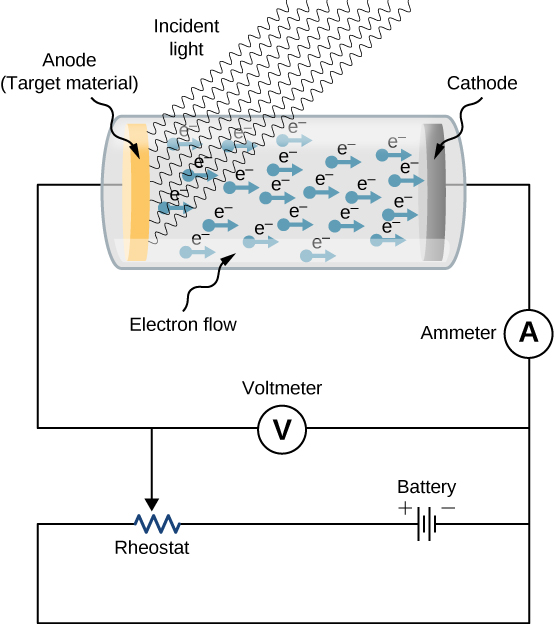
\includegraphics[width=0.5\textwidth]{Grafica/setup_fotoelettrico.jpg}
    \caption{Schema del setup per l'effetto fotoelettrico}
    \label{fig:setup_fotoelettrico}
\end{figure}
Si osserva che illuminando una lamina in un tubo a vuoto, alcuni degli elettroni che si muovono liberamente sulla superficie metallica vengono liberati. Ponendo un'altra lamina vicino alla prima si osserva allora una debole corrente tra i due elettrodi, che viene misurata da un amperometro.\\
Si può misurare l'energia degli elettroni liberati applicando alle due lamine una differenza di potenziale che si opponga al loro moto. Se al \textbf{potenziale d'arresto} $\Delta V_0$ non si rileva alcuna corrente, l'energia massima degli elettroni sarà data $e\Delta V$.\\
%Inserire figure
L'effetto sembra compatibile con la teoria classica: la luce raggiunge la lamina, ed è possibile che parte dell'energia che viene trasmessa in tale modo si trasformi in energia cinetica per qualche elettrone, che riesce così a uscire dalla superficie metallica e dirigersi verso l'altro elettrodo.\\
Questa spiegazione, tuttavia, non torna con gli esperimenti. Classicamente ci si aspetterebbe:
\begin{enumerate}
    \item un intervallo di tempo misurabile tra l'accensione della luce e l'emissione dei fotoelettroni (necessario affinché la lamina assorba sufficiente energia)
    \item una proporzionalità tra intensità e $\Delta V_0$. Usando una luce più intensa, infatti, la lamina assorbe più energia, e quindi la velocità dei fotoelettroni dovrebbe aumentare, modificando il valore del $\Delta V_0$ necessario a fermarli completamente.
\end{enumerate}
Tuttavia, gli esperimenti rivelano che:
\begin{enumerate}
    \item Non c'è alcun intervallo di tempo tra assorbimento della radiazione ed emissione dei fotoelettroni entro l'accuratezza di $10^{-9}$s, compatibilmente con l'idea che l'emissione avvenga contemporaneamente all'assorbimento della luce.\\
    Ciò non torna nemmeno dal punto di vista energetico. Illuminando una lamina monoatomica di sodio con un'intensità di $10^{-6}$W/$m^2$ è possibile misurare una corrente tra le due lamine. Tuttavia una lamina monoatomica di $1$m$^2$ di sodio ha $10^{19}$ atomi, e ci si aspetta che la radiazione incidente si divida equamente su ciascuno di essi: ogni atomo riceve perciò $10^{-25}$W. Per arrivare agli $eV$ necessari a liberare un elettrone sarebbero quindi necessari tempi nell'ordine dei mesi.
    \item Aumentando l'intensità della luce aumenta la corrente misurata, ma non varia il potenziale d'arresto $\Delta V_0$. L'unico modo per variare $\Delta V_0$ consiste invece nel modificare la \textbf{frequenza} della luce incidente: aumentandola gli elettroni sono in media più energetici. In particolare, sotto una certa frequenza $\nu_0$, specifica del materiale, nessun elettrone viene mai emesso, indipendentemente dall'intensità della radiazione.
\end{enumerate}
Einstein, riprendendo l'idea di Planck di quantizzazione dell'energia, ipotizza che anche la luce sia composta da pacchetti discreti, detti \textit{fotoni}, ciascuno di energia $h\nu$.\\
In questo modo:
\begin{enumerate}
    \item L'emissione avviene istantaneamente non appena il fotone viene assorbito dall'elettrone. L'energia non è più distribuita sull'intero fronte d'onda (che spazia tutta la superficie del materiale), ma è concentrata in singoli pacchetti.
    \item Aumentare l'intensità della sorgente significa aumentare il numero di fotoni, ma non l'energia di ciascuno di essi (che dipende dalla frequenza). Perciò l'energia massima degli elettroni liberati rimane sempre la stessa: al più sarà possibile liberare più elettroni, sviluppando una corrente maggiore.
    \item A frequenze più alte corrispondono fotoni più energetici, che possono cedere una maggiore energia agli elettroni e quindi riescono ad accelerarli maggiormente.
\end{enumerate}
Sia $\phi$ la minima energia necessaria per liberare un elettrone da un particolare materiale. Allora ad essa è associata la frequenza minima $\nu_0$ necessaria perché un fotone possa liberare un elettrone:
\[
\phi = h \nu_0
\]
Se un fotone di frequenza $\nu$ libera un certo elettrone, per conservazione dell'energia si avrà:
\[
h\nu = E_k^{max} + \phi
\]
dove $E_k^{max}$ è l'energia cinetica massima disponibile all'elettrone, che sarà quindi pari a $e\Delta V_0$, con $\Delta V_0$ il potenziale d'arresto.\\
L'energia minima $\phi$ può essere determinata sperimentalmente facendo ricorso ad un altro esperimento: l'\textbf{effetto termoionico}. Si osserva che scaldando un metallo alcuni dei suoi elettroni di superficie vengono sbalzati via. È possibile allora determinare la minima energia necessaria per liberare un elettrone, e si trova che tale energia è molto vicina a quella determinata nell'effetto fotoelettrico.

\subsection{Esperimento di Young}
La spiegazione corpuscolare della luce contrasta con l'esito di alcuni esperimenti, che suggeriscono un comportamento prettamente ondulatorio. Uno di questi è dato dall'esperienza delle due fenditure di Young.\\
Illuminando di luce monocromatica due fenditure strette e vicine tra loro si proietta su uno schermo una figura d'interferenza, caratteristica di un'interazione di tipo ondulatorio.\\
Si potrebbe suggerire che la luce sia comunque composta da particelle che si comportano "come onde" quando sono in gruppo (come le molecole sulla superficie di uno specchio d'acqua). Tuttavia, riducendo l'intensità della sorgente al punto da emettere singoli fotoni alla volta si osserva lo stesso una figura d'interferenza.\\
In tal caso, porre di fronte ad una delle due fenditure un rivelatore per determinare il percorso dei singoli fotoni modifica irreversibilmente il sistema e distrugge l'interferenza.\\
Siamo così di fronte a due comportamenti distinti e contraddittori - uno corpuscolare e uno ondulatorio - dello stesso oggetto - la luce - che non sono mai osservabili contemporaneamente. Tale idea costituisce il cosiddetto \textbf{principio di incompatibilità} di Bohr.\marginpar{Principio di incompatibilità di Bohr}

\subsection{Effetto Compton}
Un'altra conferma della natura particellare della luce deriva dall'effetto Compton.\\
Un fascio collimato di raggi X con una specifica lunghezza d'onda $\lambda$ viene fatto incidere su un bersaglio di grafite, e si misurano intensità e lunghezza d'onda del fascio deviato a vari angoli.\\
Classicamente, ci si aspetta che il campo elettrico oscillante dei raggi X faccia vibrare gli elettroni del bersaglio, che a loro volta generano un'onda elettromagnetica della stessa frequenza iniziale.\\
Sperimentalmente, invece, per angoli di deviazione $\neq 0$ si osservano due picchi di intensità, uno a $\lambda$ e uno a $\lambda' > \lambda$.\\
Compton spiegò tale risultato ipotizzando che i fotoni urtassero elasticamente contro gli elettroni del bersaglio\footnote{Sperimentalmente si osserva che $\lambda'$ non dipende dal materiale utilizzato come bersaglio. Compton ipotizzò quindi che gli urti coinvolgessero elettroni liberi. In effetti l'energia dei raggi X è molto superiore a quella della radiazione visibile, che è circa sufficiente a liberare un $e^-$ da una superficie metallica.}, cedendo quindi parte della loro energia al materiale. In tal modo i fotoni riflessi hanno minor energia, e quindi una lunghezza d'onda maggiore.\\
Analizziamo quantitativamente il fenomeno. Un fotone di momento iniziale $\vec{p}_0$ urta, lungo l'asse $x$, con un $e^-$ inizialmente fermo nel sistema di riferimento del laboratorio. Dopo l'urto il fotone viene deviato ad un angolo $\theta$ con un momento $\vec{p}_1$, e l'$e^-$ ad un angolo $\varphi$ con un momento $\vec{p}_2$.\\
Per conservazione del momento si ha $\vec{p}_0 = \vec{p}_1+\vec{p}_2$. Proiettando sugli assi si ha:
\[
\begin{cases}
p_0 = p_1\cos\theta + p_2\cos\varphi\\
p_1\sin\theta = p_2\sin\varphi
\end{cases}
\]
Per semplificare le equazioni eleviamo al quadrato e sommiamo membro a membro:
\begin{align}
\begin{cases}
(p_0-p_1\cos\theta)^2 = p_2^2\cos^2\varphi\\
p_1^2\sin^2\theta = p_2^2\sin^2\varphi 
\end{cases} &\Rightarrow \nonumber
p_0^2 + \hlc{Yellow}{p_1^2\cos^2\theta} -2p_0p_1\cos\theta + \hlc{Yellow}{p_1^2\sin^2\theta} = p_2^2\\
&\Rightarrow p_0^2 + \hlc{Yellow}{p_1^2} -2p_0p_1\cos\theta = p_2^2
\label{eqn:compton-p2}
\end{align}
Applichiamo ora la conservazione dell'energia. Sia $\mathcal{E} = cp_0$ l'energia del fotone $\gamma$ prima dell'urto, e $\mathcal{E}' = cp_1$ quella dopo l'urto. Allora otteniamo:
\begin{align}
\mathcal{E}_0 + m_ec^2 &= \mathcal{E}' + \sqrt{m_e^2c^4 + c^2p_2^2} \Rightarrow c(p_0-p_1) + m_ec^2 = \sqrt{m_e^2c^4 + c^2 p_2^2}\nonumber \\
&\xrightarrow[x^2]{} \cancel{c^2}(p_0-p_1)^2+\bcancel{m_e^2c^4} + 2m_ec^{\cancel{3}}(p_0-p_1) = \bcancel{m_e^2c^4}+\cancel{c^2}p_2^2 \nonumber\\
&\Rightarrow p_2^2 = (p_0-p_1)^2 + 2m_e c(p_0-p_1)
\label{eqn:compton-E}
\end{align}
Uguagliando (\ref{eqn:compton-p2}) e (\ref{eqn:compton-E}) si ottiene:
\begin{align}
    (p_0-p_1)^2+2m_e c(p_0-p_1) = p_0^2 + p_1^2 -2p_0p_1\cos\theta\span \\
    &\Rightarrow \cancel{p_0^2} + \bcancel{p_1^2} - 2p_0p_1 + 2m_e c(p_0-p_1) = \cancel{p_0^2}+\bcancel{p_1^2}-2p_0p_1\cos\theta\nonumber\\
    &\Rightarrow m_e c(p_0-p_1) = p_0p_1(1-\cos\theta)
\end{align}
Dividendo per $m_e c p_0 p_1$ si ottiene:
\[
\frac{1}{p_1}-\frac{1}{p_0} = \frac{1}{m_e c}(1-\cos\theta)
\]
Da $p=\mathcal{E}/c = h\nu/c = h/\lambda$ possiamo sostituire $1/p_1 = \lambda'/h$ e $1/p_0 = \lambda/h$ giungendo a:
\[
\lambda' - \lambda = \Delta\lambda = \frac{h}{m_e c}(1-\cos\theta)
\]
Lo \textit{shift} della lunghezza d'onda dovuto allo scattering di Compton dipende perciò solo dall'angolo di deviazione, e non dal materiale o dalla lunghezza $\lambda$ iniziale.\\
Tali considerazioni, tuttavia, spiegano solo il secondo picco di intensità rilevato (quello centrato attorno a $\lambda'$), ma sperimentalmente si osserva un picco anche attorno alla lunghezza d'onda $\lambda$ originale.\\
La spiegazione è che alcuni fotoni interagiscono con elettroni degli orbitali interni molto legati al nucleo, e non possiedono quindi abbastanza energia per liberarli. L'urto è come se avvenisse \textit{contro l'intero nucleo atomico}, che ha una massa equivalente molto maggiore di quella di un singolo elettrone libero (per il carbonio $M \sim 22'000 m_e$). La stessa formula restituisce quindi un $\Delta \lambda \sim 0$, non osservabile sperimentalmente.\\
In effetti, tale fenomeno di scattering che non modifica la lunghezza d'onda della radiazione incidente, è già pienamente spiegato classicamente come l'effetto del campo elettrico oscillante che accelera gli elettroni del materiale, che a loro volta producono un'altra radiazione. L'effetto è detto \textbf{scattering di Rayleigh}, è prevalente per radiazioni radio, infrarosse e nel visibile (ossia per $\lambda$ alte), ed è uno dei casi in cui predizioni classiche e quantistiche coincidono. È per $\lambda$ piccole, indicativamente per raggi X e gamma, che lo scattering Compton, di natura prettamente quantistica, si fa rilevante.

\subsection{Raggi X e radiazione di bremsstrahlung} 
%[TO DO] Inserire immagini scaricate
La natura quantistica della luce si osserva anche nel fenomeno di produzione di raggi X. In un tubo a vuoto si riscalda un elettrodo metallico, in modo da estrarre da esso elettroni per effetto termoionico. Tali elettroni sono poi accelerati da una grande differenza di potenziale (dell'ordine delle decine di $kV$), e impattano contro l'anodo, decelerando improvvisamente. Nella decelerazione vengono emessi fotoni ad alta energia, con picchi di intensità nei raggi X, detti "\textbf{bremsstrahlung}" (radiazione di frenata), in una sorta di effetto Compton al contrario.\\
Classicamente ci si aspetta che la distribuzione delle lunghezze d'onda emesse sia continua, senza alcuna lunghezza d'onda minima. D'altro canto, sperimentalmente si osserva che esiste una $\lambda_{min}$ emessa, che dipende solo dal potenziale di accelerazione (esistono anche delle linee di emissione specifiche ad alta intensità, che per ora ignoriamo).\\
Di nuovo, la spiegazione quantistica risolve il problema. Ogni fotone deve essere emesso dalla decelerazione di un singolo elettrone. Normalmente un elettrone rallenta con varie interazioni, e perciò la radiazione emessa sarà di varie frequenze, come osservato. Il caso limite è quello di un $e^{-}$ che si arresta dopo un singolo urto, cedendo l'intera sua energia al fotone prodotto. Si avrà così:
\[
e\Delta V = h\nu_{max} = \frac{hc}{\lambda_{min}} \Rightarrow \lambda_{min} = \frac{hc}{e\Delta V} = \frac{1.240\cdot 10^{-6}Vm}{\Delta V}
\]

\subsection{Diffrazione a raggi X: radiazione di Bragg} %pag. 59 Resnick
%Pag. 86 Beiser
%Pag. 102 Introduction

\section{Modelli atomici}
Sperimentalmente si osserva che facendo passare della luce attraverso un gas freddo vengono a mancare alcune determinate frequenze nella radiazione risultante.\\
Analogamente, riscaldando lo stesso gas ed esaminando lo spettro della radiazione emessa si osservano intensità molto grandi in corrispondenza delle stesse specifiche lunghezze d'onda. Si parla allora di \textbf{righe di emissione} (o assorbimento)\footnote{In realtà, ad ogni riga di assorbimento corrisponde una riga di emissione, ma in un dato momento non tutte le righe di emissione corrispondono a righe di assorbimento, e quest'ultima corrispondenza varia a seconda della temperatura del gas nell'esperimento di assorbimento.}.\\
Nel caso dell'idrogeno è possibile trovare formule sperimentali che generano le righe osservate. Un esempio è la serie di Balmer, che restituisce le righe nel visible:
\[
\lambda_n = 3645.6 \left (\frac{n^2}{n^2-4} \right ) \cdot 10^{-10}m; \quad n\in\mathbb{N}
\]
Altre formule simili furono trovate da Lyman e Paschen, e sintetizzate in un'unica formula generale da Rydberg:
\[
\frac{1}{\lambda_n}= R_H \left (\frac{1}{n^2}-\frac{1}{m^2} \right ); \quad n,m \in \mathbb{N}; \> m\geq n+1; \quad R_H = 109677.581\,cm^{-1}
\]
che per $n=1$ restituisce la serie di Lyman, per $n=2$ quella di Balmer e per $n=3$ quella di Paschen.\\

\subsection{Atomo di Thompson}
Già da tempo si sapeva che gli atomi contengono cariche negative, gli elettroni, e un ugual numero di cariche positive ben più massive, i protoni, in modo da formare un corpuscolo normalmente neutro. Non si sapeva molto, invece, sulla loro disposizione.\\
Thompson ipotizzò un modello semplice, il cosiddetto "atomo a panettone", costituito da una carica positiva distribuita sfericamente, in cui sono confinati gli elettroni, che raggiungono delle posizioni di equilibrio ben definite a seguito della loro repulsione.\\
Dando energia ad un atomo è possibile far "oscillare" gli elettroni attorno alle loro posizioni di equilibrio, ottenendo quindi l'emissione di radiazione. Tuttavia, le lunghezze d'onda previste da tale modello per le righe d'emissione non coincidono con quelle osservate sperimentalmente.\\
Consideriamo un atomo di idrogeno. Nel modello di Thompson vi è una carica positiva distribuita uniformemente in una sfera di raggio $a$ tale da bilanciare la carica dell'elettrone:
\[
V\rho = e \Rightarrow \frac{4}{3}\pi a^3 \rho = e \Rightarrow \rho = \frac{3}{4}\frac{e}{\pi a^3}
\]
Su un elettrone posto a distanza $r$ dal centro dell'atomo agisce perciò un'interazione coulombiana data da:
\[
F = -\frac{1}{4\pi\epsilon_0 r^2}e\frac{4}{3}\pi r^3 \frac{3}{4}\frac{e}{\pi a^3} = -\frac{e^2}{4\pi\epsilon_0 a^3} = -kr
\]
Se perciò l'elettrone non si trova inizialmente nella configurazione d'equilibrio ($r = 0$) inizierà ad oscillare attorno ad essa, ad una frequenza che è data da:
\[
k = \frac{e^2}{4\pi \epsilon_0 a^3} \approx 2.3\cdot 10^2 \frac{N}{m} \xrightarrow{} \nu = \frac{1}{2\pi}\sqrt{\frac{k}{m}} \Rightarrow \lambda \approx 1200 \text{\AA}
\]
Il modello di Thompson non spiega perciò le numerose linee di emissione osservate per l'idrogeno.

\subsection{Esperimento di Rutheford}
Per indagare sulla struttura interna dell'atomo, Rutheford effettuò un esperimento in cui esaminò gli angoli di deviazione di particelle $\alpha$ (nuclei di $He$) all'impatto con una sottile lamina d'oro. L'esito, fortemente in disaccordo con la previsione del modello di Thompson, portò alla nascita di un nuovo modello atomico.

\subsubsection{Atomo di Thompson}
Poiché la velocità delle particelle $\alpha$ all'impatto è dell'ordine di $2\cdot 10^7$m/s, è possibile trattare l'esperimento tramite le formule della meccanica classica.\\
%[TO DO] Inserire disegno
Quantifichiamo, utilizzando il modello di Thompson, la deviazione delle particelle attesa nell'esperimento.\\
Detto $Z$ il numero atomico dell'oro, ogni atomo contiene una carica positiva distribuita sfericamente, con densità data da:
\[
\frac{4}{3}\pi \rho a^3 = Ze \Rightarrow \rho = \frac{3}{4}\frac{Ze}{\pi a^3}
\]
Una particella $\alpha$, di carica $+2e$, al passaggio all'interno di un atomo alla distanza $r < a$ dal suo centro subisce una forza (per interazione coulombiana) data da:
\[
F = \frac{1}{4\pi\epsilon_0 r^2}(2e)\left (\frac{4}{3}\pi r^3 \right ) \frac{3}{4}\frac{Ze}{\pi a^3}) = \frac{1}{2\pi \epsilon_0}\frac{Ze^2}{a^3}r = Cr 
\]
In prima approssimazione, schematizziamo la traiettoria della particella all'interno dell'atomo con una retta. Sia allora $b$ la distanza minima tra tale retta e il centro dell'atomo, e $\theta$ l'angolo tra la normale alla traiettoria passante per il centro e il raggio che congiunge il centro alla posizione ad un dato istante della particella. Si ha allora $b = r\cos\theta$.\\
La forza trasversa si ottiene proiettando $F$ sulla normale:
\[
F_\perp = F\cos\theta = Cr\cos\theta = Cb
\]
e l'impulso associato è dato da:
\[
\Delta p_\perp = \int_0^T F_\perp dt = F_\perp T
\]
dove $T$ è l'intervallo temporale che la particella trascorre all'interno dell'atomo. Ipotizzando che la velocità di $\alpha$ resti approssimativamente costante si ha:
\[
T = \frac{2\sqrt{a^2-b^2}}{v_\alpha} = \frac{2m_\alpha}{p_\alpha}\sqrt{a^2-b^2}
\]
dove $v_\alpha$ è la velocità iniziale della particella.\\
Sostituendo nell'espressione di sopra:
\[
\Delta p_\perp = (Cb)\frac{2m_\alpha}{p_\alpha}\sqrt{a^2-b^2}
\]
L'angolo di deviazione è quindi dato da:
\[
\theta \sim \tan\theta = \frac{\Delta p_\perp}{p_\alpha} = Cb\frac{2m_\alpha}{p_\alpha^2}\sqrt{a^2-b^2}=\frac{Cb}{E_k}\sqrt{a^2-b^2}
\]
dove $E_k$ è l'energia cinetica della particella $\alpha$. Osserviamo che per $b = 0$, o per $b = a$ (corrispondenti alla particella che attraversa l'atomo lungo un diametro, o lo "sfiora" con una traiettoria tangente) la corrispondente deviazione è nulla (come ci si aspetta).\\ %Formula per la deviazione media?
Calcolando la derivata rispetto a $b$ si può trovare che la deviazione massima corrisponde quando la particella incide sull'atomo con un $b = a/\sqrt{2}$. Nel caso di atomi d'oro, con $Z = 79$, $C = \frac{1}{2\pi\epsilon_0} \frac{Ze^2}{a^3} \approx 36500$ (con $a \sim 10^{-10}$). Se l'energia cinetica delle particelle $\alpha$ è di $5$MeV si ha che la deviazione massima di un $\alpha$ dopo una sola interazione con un atomo è dell'ordine di $10^{-4}$rad.\\
Durante l'attraversamento della lamina, tuttavia, ogni particella interagisce con molti atomi. Se a ciascuna interazione viene deviata di un angolo medio $\theta_i$, la deviazione totale all'uscita, dopo $N$ interazioni, sarà data da:
\[
\theta_{tot} = \sum_{i=1}^N \theta_i
\]
Ad ogni interazione la deviazione sarà di un certo $\theta_M$ verso l'alto o il basso. Dopo molte interazioni, perciò, ci si aspetta che la deviazione totale sia attorno a $0$:
\[
\langle \theta_{tot} \rangle = 0
\]
Una stima della dispersione degli angoli di deviazione è data dallo scarto quadratico medio:
\[
\theta_{tot}^{q.m.} = \sqrt{\langle \theta_{tot}^2\rangle -\bcancel{\langle \theta_{tot}\rangle^2}}
\]
dove:
\[
\langle \theta_{tot}^2 \rangle = \langle \sum_i^N \theta_i \sum_j \theta_j \rangle = \langle \sum_{ij} \theta_i \theta_j \rangle = \langle \sum_i \theta_i^2 + \underbrace{\sum_{i\neq j}\theta_i \theta_j}_{\to 0} \rangle = \langle \sum_i \theta_i^2 \rangle = N\theta_M^2 
\]
Poiché $\theta$ assume valori pari a $+\theta_M$ e $-\theta_M$ con ugual probabilità, si ha che il prodotto $\theta_i\theta_j$ sarà il $50\%$ delle volte positivo e il $50\%$ delle volte negativo: il suo valor atteso sarà perciò nullo.\\
Nel caso di una lamina sottile il numero di atomi attraversati da ogni particella $\alpha$ è dell'ordine di $10^4$, e la dispersione è perciò:
\[
\theta_{tot}^{q.m.} = \sqrt{N}\theta_M \sim 10^{-2}rad = 0.6^\circ
\]
Ci si aspetta perciò che il fascio di particelle venga solo leggermente deviato.\\
La deviazione massima, che si ha nel caso una particella venga deviata sempre nella stessa direzione, è dell'ordine di $N\theta_M \sim 1$rad $\sim 60^\circ$, e avviene con una probabilità di $(1/2)^N \sim 10^{-3000}$. Per confronto, il numero di atomi nell'universo osservabile è stimato tra $10^{78}$ e $10^{82}$.\\
Sperimentalmente, tuttavia, si rilevano deviazioni molto alte con una probabilità significativa, ossia dei risultati completamente incompatibili con quanto previsto dal modello di Thompson.

\subsubsection{Atomo di Rutheford}
Per spiegare le ampie deviazioni rilevate dall'esperimento, Rutheford propose un nuovo modello atomico, in cui l'intera carica positiva è concentrata in una regione sferica molto ristretta (il \textbf{nucleo}), e le cariche negative (elettroni) vi ruotano attorno, come in una specie di sistema planetario in miniatura.\\
Esaminiamo allora, quantitativamente, quale sia la deviazione attesa per le particelle $\alpha$ in questo caso.
\begin{figure}[H]
    \centering
    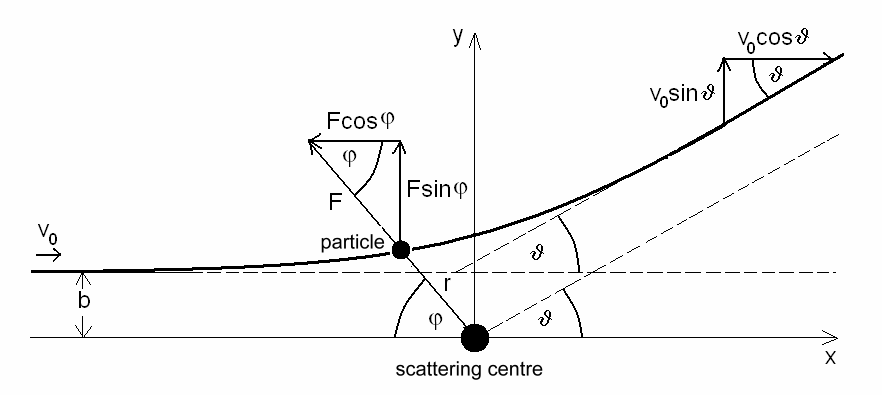
\includegraphics[scale=0.6]{Grafica/RuthefordSdr.png}
    \caption{Esperimento di Rutheford}
    \label{fig:rutheford}
\end{figure}%[TO DO]Sistemare questa figura coerentemente con quanto mostrato nel testo (togliere 0 a v_0 e sistemare l'angolo $\varphi$)
Uno schema di una singola interazione è presentato in figura \ref{fig:rutheford}. L'atomo d'oro si trova all'origine di un sistema di riferimento cartesiano, e una particella $\alpha$ di carica $+2e$ con velocità iniziale $\vec{v} = v\hat{x}$, inizialmente a distanza $b \geq 0$ (parametro d'impatto) dall'asse $\hat{x}$, giunge da molto lontano e interagisce in modo coulombiano con il nucleo atomico, subendo una deviazione di un angolo $\theta$.\\
Consideriamo le seguenti semplificazioni:
\begin{itemize}
    \item L'atomo centrale rimane completamente fermo nel sistema di riferimento del laboratorio nel corso di tutta l'interazione (giustificata dal fatto che $M_\text{nucleo} \gg m_\alpha$)
    \item L'energia delle particelle $\alpha$ incidenti è sufficientemente bassa da consentire la trattazione tramite la meccanica classica
    \item Le particelle giungono sufficientemente vicino al nucleo, ossia $b$ è vicino a $0$. In questo modo possiamo ignorare la presenza degli elettroni che circondano l'atomo d'oro, e le cui cariche negative schermano parzialmente la carica positiva centrale.
\end{itemize}
L'interazione è schematizzabile come un urto elastico. Detta $v$ la velocità prima dell'urto e $v'$ quella dopo, per conservazione dell'energia si ha:
\[
\frac{1}{2}mv^2 = \frac{1}{2}mv'^2 \Rightarrow v' = v
\]
Si conserva anche il momento angolare rispetto all'origine (posizione dell'atomo d'oro):
\[
mv b = mv'b' = m\omega r^2 \Rightarrow \omega = \frac{v b}{r^2}
\]
dove $\omega$ è la velocità angolare della particella, ossia $d\varphi/dt$ per una qualsiasi coordinata angolare $\varphi$ rispetto all'origine.\\
%[TO DO] Inserire figura regola del parallelogramma
Prima dell'urto il momento è $\vec{p}_1 = p_1 \hat{x}$, mentre dopo è $\vec{p}_2$, di stesso modulo $|\vec{p}_1|=|\vec{p}_2|=p$ (in quanto $v' = v$), ma ad angolo $\theta$ rispetto a $+\hat{x}$). Ricavando l'impulso $\Delta \vec{p}$ per regola del parallelogramma si ha che il triangolo di lati $p_1$, $p_2$ e $\Delta p$ è isoscele sulla base $\Delta p$, e l'angolo al vertice (tra $p_1$ e $p_2$) è pari a $\theta$. Perciò $\Delta \vec{p}$ forma un angolo di $(\pi-\theta)/2$ con $-\hat{x}$. Applicando il teorema dei seni:
\begin{equation}
\frac{\Delta p}{\sin\theta} = \frac{\hlc{Yellow}{p}}{\sin \left ( \frac{\pi-\theta}{2} \right )} \Rightarrow \Delta p = \frac{\hlc{Yellow}{mv}\sin\theta}{\sin \left ( \frac{\pi-\theta}{2}\right )} \underset{(*)}{=} \frac{2mv\sin\frac{\theta}{2}\cos\frac{\theta}{2}}{\cos\frac{\theta}{2}} = 2mv\sin\left (\frac{\theta}{2}\right ) 
\label{eqn:ruth-deltap1}
\end{equation}
Dalla dinamica si ha che:
\[
\Delta p = \left |\int_{-\infty}^{+\infty} \vec{F}dt \right |
\]
dove $\vec{F}$ è la forza derivante dall'interazione coulombiana. Per svolgere l'integrale proiettiamo il modulo di $F$ lungo la direzione di $\Delta \vec{p}$. Sia $\varphi$ l'angolo tra $\Delta \vec{p}$ e il raggio vettore che congiunge l'origine alla posizione della particella $\alpha$ ad un dato istante. Nel corso dell'interazione si ha allora che $\varphi$ assume valori compresi tra $-\frac{\pi-\theta}{2}$ e $+\frac{\pi-\theta}{2}$. Passando quindi alla variabile angolare $\varphi$ all'interno dell'integrale:
\[
\Delta p = \int_{-\infty}^{+\infty} F\cos\varphi dt = \int_{-\frac{\pi-\theta}{2}}^{\frac{\pi-\theta}{2}} \hlc{ForestGreen}{F}\cos\varphi \hlc{SkyBlue}{\frac{dt}{d\varphi}}d\varphi 
\]
dove $\frac{dt}{d\varphi} = (d\varphi/dt)^{-1} = \omega^{-1} = r^2/vb$ (come ricavato dalla conservazione del momento angolare).\\
$F$ ha poi l'espressione della forza di Coulomb, ed è quindi pari a $2Ze^2/(4\pi\epsilon_0 r^2)$. Sostituendo tutto nell'integrale si giunge a:
\begin{equation}
\Delta p = 
\int_{-\frac{\pi-\theta}{2}}^{\frac{\pi-\theta}{2}} \hlc{ForestGreen}{\frac{2Z e^2}{4\pi\epsilon_0 r^2}}\hlc{SkyBlue}{\frac{r^2}{vb}} \cos\varphi\,d\varphi = \frac{Ze^2}{2\pi\epsilon_0 v b} \left[\sin\varphi \right ]_{\frac{\pi-\theta}{2}}^{\frac{\pi-\theta}{2}} = \frac{Ze^2}{\pi\epsilon_0 v b}\sin\left ( \frac{\pi-\theta}{2}\right )
\label{eqn:ruth-deltap2}
\end{equation}
Uguagliando i risultati ottenuti in (\ref{eqn:ruth-deltap1}) e (\ref{eqn:ruth-deltap2}) si giunge a:
\begin{equation}
2mv\sin\left ( \frac{\theta}{2}\right ) = \frac{Ze^2}{\pi\epsilon_0v b}\sin\left ( \frac{\pi-\theta}{2}\right ) \Rightarrow \frac{2\pi\epsilon_0}{Ze^2}mv^2b \sin\left ( \frac{\theta}{2}\right ) = \sin\left ( \frac{\pi-\theta}{2}\right )
\label{eqn:deltap-eq1}
\end{equation}
Dalla goniometria:
\[
\sin\left ( \frac{\pi-\theta}{2}\right ) = \sin\left ( \frac{\pi}{2}-\frac{\theta}{2}\right ) = \cos\left (\frac{\theta}{2}\right )
\]
Sostituendo in (\ref{eqn:deltap-eq1}) e dividendo entrambi i membri per $\cos(\theta/2)$ si giunge a:
\begin{equation}
\cot\left( \frac{\theta}{2}\right ) = \frac{4\pi\epsilon_0}{Ze^2} \hlc{Yellow}{\frac{mv^2}{2}}b = \frac{4\pi\epsilon_0}{Ze^2}\hlc{Yellow}{E_k} b \Rightarrow b = \frac{Ze^2\cot\frac{\theta}{2}}{4\pi\epsilon_0}E_k
\label{eqn:rutheford-b-theta}
\end{equation}
Abbiamo quindi ottenuto una relazione tra il parametro di impatto $b$ e l'angolo $\theta$ di deviazione risultante. Esaminando la funzione si nota che $\theta$ diviene molto alto per $b$ particolarmente piccoli, e ciò potrebbe spiegare le osservazioni sperimentali.\\
Consideriamo ora l'interazione con l'intera lamina. Poiché le deviazioni ampie sono relativamente rare, possiamo lavorare nell'ipotesi che ogni particella $\alpha$ interagisca al più con un solo atomo lungo la sua traiettoria. Tale assunzione sarà giustificata a posteriori dal fatto che il nucleo atomico è molto più piccolo delle dimensioni utilizzate, per esempio, nel modello di Thompson.\\
Abbiamo visto che se una particella raggiunge un atomo con un parametro d'impatto $b$ sarà deviata ad un angolo $\theta$. Tutte le particelle che entrano nell'atomo con un $b$ minore, ossia le cui traiettorie intersecano un cerchio di raggio $b$ centrato sull'atomo, saranno allora deviate ad un $\bar{\theta} > \theta$.\\
Rappresentiamo quindi la lamina come una superficie rettangolare su cui sono disposti uniformemente i "cerchi di interazione" di ogni atomo. Se una particella in arrivo colpisce l'interno di uno di questi cerchi sarà deviata ad un angolo maggiore di $\theta$, e la probabilità che ciò succeda è pari al rapporto tra l'area totale dei cerchi e l'area della lamina stessa.\\
Detta $n$ la densità atomica della lamina, ossia il numero di atomi per unità di volume, in una lamina di superficie $A$ e spessore $t$ vi saranno $n(At)$ atomi. Sia ora $\sigma$ l'area di ogni "cerchio di interazione" (di raggio $b$). La frazione $f_{>\theta}$ di urti che portano ad una deviazione maggiore di $\theta$ (ossia degli urti che colpiscono i cerchi) è quindi:
\[
f_{>\theta} = \frac{nAt \sigma}{A} = nt\hlc{Yellow}{\sigma} = nt(\hlc{Yellow}{\pi b^2})
\]
Ricavando $b$ dalla (\ref{eqn:rutheford-b-theta}) e sostituendolo nell'espressione sopra si ottiene:
\begin{equation}
f_{>\theta} = nt\pi \left ( \frac{Ze^2}{4\pi\epsilon_0} \right )^2 \frac{1}{E_k^2} \cot^2\left ( \frac{\theta}{2}\right )
\label{eqn-rutheford-fraction}
\end{equation}
ossia un'espressione per la frazione di particelle che vengono deviate ad un angolo maggiore di $\theta$ in funzione dell'angolo $\theta$ stesso.

\textbf{Esempio numerico} Per $E_k = 7.7$MeV, $t = 3\cdot 10^{-7}$m e $\rho = 1.93\cdot 10^4$ kg/$m^3$, $Z = 79$, si ottiene $n = \rho/m_{\text{atomo}} = 5.9 \cdot 10^{28}$ m$^{-3}$, da cui $f_{>45^\circ} \approx 7\cdot 10^{-5} = 0.007 \%$: la probabilità di deviazioni grandi è perciò significativa, diversamente dal caso di Thompson.\\
\begin{figure}[H]
    \centering
    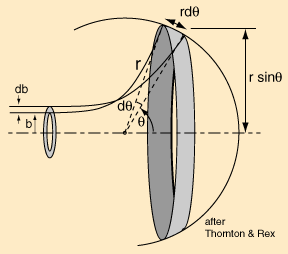
\includegraphics{Grafica/Ruthcross.png}
    \caption{Sezione trasversa differenziale}
    \label{fig:rutheford-cross-section}
\end{figure}

Troviamo ora una relazione differenziale che dia la frazione di particelle tra un angolo $\theta$ e $\theta+d\theta$.
Per trovare la frazione di particelle che vengono deviate tra $\theta$ e $\theta+d\theta$ basta differenziare la (\ref{eqn-rutheford-fraction}):
\[
df = -nt\pi \left ( \frac{Ze^2}{4\pi\epsilon_0} \right )^2 \frac{1}{E_k^2} 2\cot\left ( \frac{\theta}{2}\right ) \frac{1}{\sin^2\frac{\theta}{2}}\frac{d\theta}{2} = -nt\pi \left ( \frac{Ze^2}{4\pi\epsilon_0}\right )^2 \frac{1}{E_k^2} \frac{\cos\frac{\theta}{2}}{\sin^3\frac{\theta}{2}}d\theta
\]
e prenderne il valore assoluto\footnote{Il segno negativo nel differenziale compare poiché all'aumentare dell'angolo di deviazione la probabilità cala - come ci si aspetta}.\\
Se lo schermo (sferico) del rilevatore è posizionato a distanza $r$ dall'origine, allora l'area su cui tali particelle si distribuiscono è quella evidenziata in figura \ref{fig:rutheford-cross-section}, pari a:
\[
dS = (2\pi r \sin\theta)(r d\theta) = 2\pi r^2 \sin\theta d\theta = 4\pi r^2 \sin\left ( \frac{\theta}{2}
\right ) \cos\left ( \frac{\theta}{2} \right )
\]
Se inizialmente vengono lanciate $N_i$ particelle, allora il numero (medio) di particelle \textit{per unità d'area} che colpiscono il rivelatore tra $\theta$ e $\theta+d\theta$, dopo aver superato una lamina di spessore $t$ con una densità $n$ di atomi di numero atomico $Z$ è dato da:
\[
\frac{N(\theta)}{A} = N_i\frac{|df|}{dS} = \frac{n t N_i}{r^2} \left (\frac{Z e^2}{8\pi \epsilon_0} \right )^2 \frac{1}{E_k^2} \frac{1}{\sin^4 \frac{\theta}{2}}
\]
Il numero di particelle per steradiante (unità d'angolo solido) si ottiene dividendo $|df|$ per $d\Omega = dS/r^2$, ed è pari a:
\[
\mathcal{N}(\theta) = N_i\cdot (nt) \cdot \frac{d\sigma}{d\Omega}; \quad \frac{d\sigma}{d\Omega} = \left ( \frac{Ze^2}{8\pi\epsilon_0} \right )^2 \frac{1}{E_k^2}\frac{1}{\sin^4 \frac{\theta}{2}} 
\]
dove $nt$ può essere visto come il numero di atomi per unità d'area sulla lamina, mentre $d\sigma/d\Omega$ è detta \textbf{sezione trasversa differenziale}\footnote{Sui testi inglesi: \textit{differential cross-section}}.\\
La distribuzione così trovata è in perfetto accordo con i dati sperimentali per $E_k$ sufficientemente bassa (per cui si possono trascurare gli effetti relativistici).\\
Tuttavia vengono osservate deviazioni dalla teoria anche per valori non relativistici, specialmente nel caso di nuclei leggeri come bersaglio\footnote{Anche dopo aver riadattato la formula a questo caso, che non è attualmente previsto nelle nostre ipotesi in quanto il nucleo viene supposto sempre fermo.}.\\
Nel dettaglio, sia $R_{min}$ la distanza di minimo avvicinamento al nucleo, che si ottiene nel caso di impatto diretto (con deviazione di $180^\circ$, per cui la particella lanciata torna completamente indietro). A $R_{min}$ l'energia cinetica di $\alpha$ è nulla, e si è convertita completamente in energia potenziale elettrostatica:
\[
E_k = \frac{2Ze^2}{4\pi\epsilon_0 R_{min}} \Rightarrow R_{min} = \frac{2Ze^2}{4\pi\epsilon_0 E_k}
\]
L'accordo tra teoria ed esperimento è quantificato da $N(\theta)_{th.}/N(\theta)_{sper.}$. Graficando tale rapporto in funzione di $R_{min}$ (che è dato dall'energia cinetica utilizzata per le particelle incidenti), ci si accorge che il valore è prossimo a $1$ (ottimo accordo) fino a $10^{-14}$m. Per raggi minori si rilevano invece deviazioni significative.\\
La spiegazione è data dal fatto che il modello considera interazioni puramente elettrostatiche: se però le particelle $\alpha$ sono sufficientemente energetiche possono verificarsi casi in cui esse entrano nella regione nucleare, dove agiscono forze di interazione differenti. L'esperimento di Rutheford, perciò, consente di dare anche una stima della grandezza del nucleo atomico, corrispondente al primo valore al quale si verificano deviazioni dalla teoria.\\
Osservando che la dimensione del nucleo è di $4$ ordini di grandezza più piccola del raggio atomico si giustifica l'ipotesi che ogni particella $\alpha$ interagisca con al più un atomo durante la sua traiettoria.

\marginpar{Problemi}Il modello di Rutheford non è però esente da problemi: se gli elettroni ruotano attorno al nucleo allora devono emettere radiazione, in quanto cariche elettriche accelerate. Ma allora devono perdere energia, e quindi spiraleggiare verso il nucleo, rendendo gli atomi instabili. Se il modello di Rutheford fosse vero, perciò, tutta la materia si dovrebbe disintegrare nel giro di una frazione di secondo, cosa che è evidentemente inesatta.\\
È per risolvere questo problema che Bohr sviluppò un nuovo modello, in cui anche il momento angolare degli elettroni è quantizzato, e perciò sono possibili solo certe orbite e non tutte.

\subsection{Teoria atomica di Bohr}
Il modello di Bohr parte dalle seguenti ipotesi:
\begin{enumerate}
    \item Gli elettroni si muovono attorno al nucleo in orbite \textbf{circolari stabili}, sotto l'influsso dell'interazione coulombiana e obbedendo alle leggi della meccanica classica (l'approssimazione $v \ll c$ è considerata valida).
    \item \textbf{Quantizzazione} Non tutte le orbite sono possibili, ma solo quelle con certi valori del momento angolare orbitale $L = n\hbar$, $n \in \mathbb{N}$ e $\hbar = h/(2\pi)$.
    \item Ogni elettrone, pur essendo in constante accelerazione, non emette radiazione, e perciò la sua energia $\mathcal{E}$ rimane costante. Ciò è motivato dal fatto che si osserva sperimentalmente la stabilità degli atomi
    \item Se un elettrone passa da un'orbita a energia $\mathcal{E}_i$ a una con energia $\mathcal{E}_f$ in maniera discontinua (con un "salto", in quanto i valori intermedi non sono permessi) allora emetterà un fotone ad una frequenza $\nu = (\mathcal{E}_i-\mathcal{E}_f)/h$. Ciò deriva dal lavoro di Einstein sull'effetto fotoelettrico.
\end{enumerate}
Nell'approssimazione che la massa degli elettroni sia molto minore di quella del nucleo (generalmente valida), si può considerare il nucleo completamente fisso\footnote{In realtà i due dovrebbero "orbitare" attorno al loro centro di massa, come nel caso di Terra e Sole}. Allora la forza di Coulomb agisce da forza centripeta:
\begin{equation}
\frac{Ze^2}{4\pi\epsilon_0 r^2} = \frac{m v^2}{r} \Rightarrow \frac{Ze^2}{4\pi\epsilon_0} = mv^2 r
\label{eqn:bohr-bilanciamento}
\end{equation}
con $m$ la massa dell'elettrone.\\
Dalla condizione di quantizzazione si ricava che non tutte le velocità sono ammesse:
\[
mvr = n\hbar \Rightarrow v = \frac{n\hbar}{mr}
\]
Sostituendola nella (\ref{eqn:bohr-bilanciamento}) si ottiene:
\[
\frac{1}{4\pi\epsilon_0}Ze^2 = \frac{m n^2 \hbar^2}{m^2 r^2}r \Rightarrow r_n = 4\pi\epsilon_0\frac{n^2 \hbar^2}{m Z e^2}; \quad v_n = \frac{1}{4\pi\epsilon_0}\frac{Ze^2}{n\hbar}
\]
Per $Z = 1$ si ottiene $r_1 = 5.3\cdot 10^{-11}$m $\approx 0.5$\AA, in accordo con le stime sperimentali. Per la velocità si ha $v_1 \approx 2.2. \cdot 10^6$m/s, pari a meno dell'$1\%$ di $c$: si giustifica quindi l'approssimazione della meccanica classica. Infatti:
\[
\frac{v_1}{c} = \frac{e^2}{4\pi\epsilon_0 \hbar c} = \alpha \sim \frac{1}{137}
\]
dove $\alpha$ è la \textbf{costante di struttura fine}, una costante adimensionale importante in fisica teorica.\\
Chiaramente, per valori di $Z$ alti le velocità entrano nel regime relativistico, e il modello di Bohr non può più essere applicato.\\
Fissata a $0$ l'energia dell'elettrone quando è posto a distanza infinita dal nucleo, a distanza $r$ si ha:
\[
V = -\int_r^\infty \frac{Ze^2}{4\pi\epsilon_0 r^2}dr = -\frac{Ze^2}{4\pi\epsilon_0 r}
\]
L'energia cinetica per l'orbita che passa per $r$ si ricava da (\ref{eqn:bohr-bilanciamento}) dividendo entrambi i membri per $2r$:
\[
\frac{Ze^2}{4\pi\epsilon_0} = mv^2 r \Rightarrow \frac{Ze^2}{8\pi\epsilon_0} = \frac{1}{2}mv^2 = K
\]
L'energia totale dell'elettrone è perciò:
\[
\mathcal{E} = V + K = -\frac{Ze^2}{8\pi\epsilon_0 r} = -K
\]
E sostituendo $r$ al suo interno si giunge a:
\[
\mathcal{E}_n = -\frac{mZ^2 e^4}{2(4\pi\epsilon_0)^2\hbar^2}\frac{1}{n^2}
\]
Perciò quantizzare il momento angolare dell'elettrone conduce a quantizzare anche la sua energia.\\
Quando un elettrone passa da un livello $n_i$ a un livello $n_f$, con $n_i \neq n_f$, si ha l'emissione di un fotone ad una certa frequenza $\nu$, che sarà data da:
\[
\nu_{i\to f} = \frac{\mathcal{E}_i-\mathcal{E}_f}{h} = \frac{mZ^2 e^4}{2(4\pi\epsilon_0)^2 \hbar^2 h}\left ( \frac{1}{n_f^2}-\frac{1}{n_i^2} \right )
\]
Per l'idrogeno $Z = 1$ e si ha:
\[
\frac{1}{\lambda} = \frac{\nu_{i\to f}}{c} = \frac{m \hlc{Yellow}{e^4}}{2hc \hlc{Yellow}{(4\pi\epsilon_0)^2 \hbar^2}}{\color{Blue}\frac{c^2}{\hlc{Yellow}{c^2}}} \left ( \frac{1}{n_f^2}-\frac{1}{n_i^2}\right ) = \frac{c \hlc{Yellow}{\alpha^2} m}{2h}\left ( \frac{1}{n_f^2}-\frac{1}{n_i^2}\right )
\]
si ottiene cioè la formula di Rydberg, da cui:
\[
R_h = \frac{c\alpha^2 m}{2h}
\]
Se per $m$ si usa semplicemente la massa dell'elettrone si ottiene tuttavia un valore leggermente diverso da quello sperimentale:
\[
R_h^{th.} = 109'737.268\,\text{cm}^{-1}; \quad R_h^{sper.} = 109'677.581\,\text{cm}^{-1}
\]
ma basta usare la massa ridotta del sistema $\mu = mM/(m+M)$, con $M$ massa del nucleo, (rimuovendo l'approssimazione di nucleo stazionario) per ridurre la discrepanza e ottenere ${R_h^{th}}' = 109'677.531$ cm$^{-1}$ in perfetto accordo con gli esperimenti.\\
La formula trovata da Bohr spiega ottimamente lo spettro dell'idrogeno e di sostanze leggere nello stato in cui hanno un solo elettrone (come nel caso di un gas di elio ionizzato $He^+$), ma non quelle di atomi più pesanti (dove vi sono fenomeni di interazione tra gli elettroni che non sono qui modellizzati).\\
Infatti, un atomo di idrogeno può assorbire un fotone solo se la sua frequenza è tale da garantire il passaggio di un elettrone ad uno dei livelli superiori: vi è quindi solo un discreto numero di possibilità. Inoltre, se si illumina un gas di idrogeno freddo, la maggior parte degli elettroni sarà allo stato più basso (con $n=1$) e perciò si osserveranno solo le righe che corrispondono a stati di partenza $n_i = 1$. Riscaldando il gas, gli urti tra atomi diversi hanno la possibilità di spingere elettroni a stati più elevati, e si possono quindi osservare transizioni da $n_i > 1$.

\subsection{Esperimento di Franck-Hertz}
Una conferma diretta della quantizzazione dell'energia degli elettroni nell'atomi è data dall'esperimento di Franck-Hertz.\\
In un tubo contenente gas di mercurio a bassa pressione sono posizionati due elettrodi, tra i quali viene impostata una differenza di potenziale $\Delta V$. Riscaldando il primo elettrodo vengono liberati degli elettroni, che sono accelerati dalla differenza di potenziale verso l'anodo, su cui sono praticati dei fori. Alcuni elettroni passano quindi attraverso il secondo elettrodo ed entrano in una regione in cui si ha una differenza di potenziale opposta, che li rallenta. Un terzo elettrodo raccoglie gli elettroni in grado di superare quest'ultimo potenziale, e tramite un amperometro si misura la corrente così generata.\\
%[TO DO] Inserire immagini
Aumentando la $\Delta V$ di accelerazione inizialmente aumenta anche la corrente misurata. Quando però $\Delta V$ raggiunge i $4.9$V la corrente cala di colpo, per poi tornare a salire man mano che si continua ad aumentare $\Delta V$.\\
La spiegazione di ciò sta nel fatto che gli atomi di mercurio possono assorbire energia solo in "pacchetti fissati". Solo gli elettroni con la giusta energia possono perciò eccitare gli atomi di $Hg$, cedendo la loro energia cinetica nel processo.\\
Osservando lo spettro del mercurio si nota poi la comparsa di una riga di emissione solo quando $\Delta V$ è appena oltre a $4.9$V, e non prima. Tale linea è poi compatibile con fotoni di energia pari a $4.9$eV, in pieno accordo con il modello di Bohr.\\
Se si continua ad aumentare $\Delta V$ è possibile osservare ulteriori momenti in cui la corrente si annulla, corrispondenti a multipli di $4.9$V (per cui gli elettroni possono urtare un $Hg$ e guadagnare abbastanza energia per urtarne un altro), oppure ad altre energie che possono essere assorbite dal mercurio (corrispondenti a salti tra $n_i = 1$ e $n_f > 2$).

\subsection{Quantizzazione di Sommerfield}
Qual è la relazione tra la quantizzazione del momento angolare introdotta da Bohr e quella dell'energia delle onde stazionarie dovuta a Planck?\\
Nel 1916 Wilson e Sommerfield definirono un insieme di regole per la quantizzazione di sistemi fisici, da cui si potevano derivare le formule di Bohr e Planck come casi speciali.\\
\marginpar{Quantizzazione}L'idea è che per ogni sistema fisico le cui coordinate sono funzioni periodiche del tempo, esiste una \textit{condizione di quantizzazione} per ciascuna delle coordinate $q$, della forma di:
\[
\oint p_q dq = n_q h
\]
dove $p_q$ è il momento associato a quella coordinata, $n_q$ è un numero intero e l'integrazione è intesa su un intero periodo della coordinata $q$.\\
Nel caso di un oscillatore armonico, l'energia totale è:
\[
E = K + V = \frac{p_x^2}{2m}+\frac{kx^2}{2} \Rightarrow \frac{p_x^2}{2mE} + \frac{x^2}{2E/k} = 1
\]
Rappresentando questa relazione su un piano cartesiano con assi $(x,p_x)$ (detto spazio delle fasi) si ottiene un ellisse di semiassi $a = \sqrt{2E/k}$ e $b = \sqrt{2mE}$. Un punto su questo piano corrisponde ad uno stato di un sistema in un dato istante. Durante una completa oscillazione il punto percorre nello spazio delle fasi una traiettoria ellittica.\\
Osservando che l'integrale della condizione di quantizzazione equivale all'area dell'ellisse si ha:
\[
\oint p_x dx = \pi a b = \frac{2\pi E}{\sqrt{k/m}}
\]
Sostituendo $\sqrt{k/m} = 2\pi\nu$ (frequenza di un oscillatore armonico) ed uguagliando alla condizione di quantizzazione:
\[
\oint p_x dx = \frac{E}{\nu} = n_x h \Rightarrow E = nh\nu
\]
Si ottiene perciò la quantizzazione di Planck.\\
Se invece consideriamo un elettrone che percorre un'orbita circolare di raggio $r$ a momento angolare costante, si ha che la coordinata angolare $\theta$ è periodica (va da $0$ a $2\pi$ e poi ricomincia da capo). Applicando allora la condizione di quantizzazione:
\[
\oint p_q\,dq = n_q h \Rightarrow \oint L\,d\theta = nh 
\]
dove
\[
\oint L\,d\theta = L \int_0^{2\pi} d\theta = 2\pi L
\]
e perciò:
\[
2\pi L = nh \Rightarrow L = \frac{nh}{2\pi} = n\hbar
\]
ossia la quantizzazione di Bohr.

\subsection{Atomo di Sommerfield}
Osservazioni sperimentali di precisione consentono di determinare che le righe della serie dell'idrogeno (e di tutti gli altri elementi) non sono in realtà \textit{singole}, ma \textit{doppie} o \textit{multiple}, con una separazione tra di esse di $10^4$ volte inferiore rispetto a quella tra una riga "principale" e la successiva. Tali righe "sdoppiate" fanno parte della cosiddetta \textbf{struttura fine} dello spettro atomico.\\
Ciò significa che quello che prima si pensava essere un singolo stato è in realtà composto da più stati di energie molto simili tra loro. Sommerfield ipotizzò che le orbite degli elettroni attorno al nucleo fossero ellittiche e non circolari. Usando coordinate polari $r$ e $\theta$ si hanno due condizioni di quantizzazione, una sul momento angolare (corrispondente a $\theta$) e una, non presente nel caso di Bohr in cui $r$ è costante, sul momento radiale. Si hanno quindi due numeri quantici: $n_r$ e $n_\theta$.\\
Detto $n = n_r + n_\theta$, l'analisi di Sommerfield porta ai seguenti valori per i semiassi delle orbite e per la loro energia:
\[
a = \frac{4\pi\epsilon_0 n^2 \hbar^2}{\mu Z e^2} = r_n; \quad b = a \frac{n_\theta}{n}; \quad E = -\left ( \frac{1}{4\pi\epsilon_0} \right )^2 \frac{\mu Z^2 e^4}{2n^2 \hbar^2} = E_n
\]
Fissato $n$, $n_r$ può assumere valori tra $0$ e $n$, e $n_\theta$ tra $1$ e $n$. Se $n_r = n$ l'orbita è circolare, come nell'atomo di Bohr. Per ogni $n$, tuttavia, vi sono $n$ possibili orbite, che hanno tutte la stessa energia (e per questo vengono dette \textit{degeneri}).\\
Per produrre la piccola differenza di energia tra tali stati, in modo da spiegare la struttura fine dell'idrogeno, è necessario utilizzare le formule della relatività, abbandonando la semplificazione della meccanica classica.\\
Così facendo, Sommerfield ottenne una formula capace di spiegare con buona accuratezza gli esperimenti. Tale modello, tuttavia, prevede transizioni che non vengono mai osservate: è necessario quindi inserire un'ulteriore condizione, per cui un elettrone può passare ad un altro livello se e solo se $n_{\theta i}-n_{\theta f} = \pm 1$. Tale restrizione è detta \textbf{regola di selezione}.
%Inserire figura e ref. a pag 116 del Reisnick

\subsection{Principio di corrispondenza}
Bohr giustificò la comparsa di regole di selezione con il \textbf{principio di corrispondenza}: %[TO DO] Rimuovere il precedente enunciato fatto un po' così
\begin{enumerate}
    \item Le predizioni della meccanica quantistica devono corrispondere a quelle della fisica classica nel limite in cui i numeri quantici che specificano lo stato del sistema diventano grandi. 
    \item Una regola di selezione deve valere sempre: sia per $n$ grandi (limite classico) che per $n$ piccoli (limite quantistico).
\end{enumerate}
L'idea dietro al primo principio sta dietro al caso della radiazione di corpo nero, per cui la formula di Rayleigh-Jeans (puramente classica) approssima fedelmente gli esperimenti per $\nu \to 0$. Infatti in questo caso $\mathcal{E} = nh\nu \to kT = \text{const.}$, per cui abbassando $\nu$, $n \to +\infty$. Si può quindi considerare la corrispondenza numeri quantici alti $\to$ sistema si comporta "classicamente".\\
Il principio di corrispondenza è soddisfatto completamente da sistemi semplici, come un pendolo carico che compie un moto armonico\footnote{Una dimostrazione discorsiva è data a pag. 117 dell'Eisberg-Resnick, al capitolo 4-11.}.\\
Proviamo ad applicarlo nel caso dell'analisi dello spettro di un atomo di idrogeno.\\
Dall'elettromagnetismo classico si ha che un elettrone in moto circolare emette una radiazione di frequenza pari a quella di rivoluzione. Dalle formule trovate per l'atomo di Bohr si ha quindi:
\[
\nu_0 = \frac{v}{2\pi r} = \left ( \frac{1}{4\pi\epsilon_0} \right )^2 \frac{me^4}{2\pi(n\hbar)^3 } = -\frac{2\mathcal{E}_1}{h\,n^3}; \quad \mathcal{E}_1 = -\frac{me^4}{2(4\pi\epsilon_0)^2 \hbar^2}; \> \hbar = \frac{h}{2\pi}
\]
Nel caso quantistico, come già ricavato, si ha:
\[
\nu_{i\to f} = \frac{mZ^2 e^4}{2(4\pi\epsilon_0)^2\hbar^2 h}\left ( \frac{1}{n_f^2}-\frac{1}{n_i^2} \right ) = -\frac{\mathcal{E}_1}{h}\left (\frac{1}{n_f^2}-\frac{1}{n_i^2}\right )
\]
Considerando una transizione da $(n-p) \to n$:
\[
\nu_{\Delta p} = -\frac{\mathcal{E}_1}{h}\left ( \frac{1}{n^2}-\frac{1}{(n-p)^2} \right ) = -\frac{\mathcal{E}_1}{h}\frac{p(p-2n)}{n^2(n-p)^2}
\]
Nel limite per $n\to +\infty$, in approssimazione al primo termine si ha:
\[
\nu_{\Delta p} \approx -\frac{2n \mathcal{E}_1 p}{h n^4} = -\frac{2 \mathcal{E}_1 p}{h n^3}
\]
che equivale al caso classico se imponiamo $p = 1$, ossia limitando le transizioni possibili a quelle tra un livello e il livello appena superiore. Questa diviene quindi una \textbf{regola di selezione}.\\
\marginpar{Problemi del modello di Bohr}Ci aspettiamo che tale restrizione valga sia nel caso classico che in quello quantistico. Tuttavia, sperimentalmente, si osservano transizioni con $\Delta n > 1$ per $n$ bassi.
Nel caso dell'atomo di idrogeno il principio di corrispondenza non è perciò sufficiente a garantire il pieno accordo tra teoria e realtà, neanche considerando i tentativi di Sommerfield.

\subsection{I problemi della old quantum theory}
I modelli di Bohr e Sommerfield, nonostante grandi successi sperimentali, presentano delle significative incompletezze:
\begin{itemize}
    \item Non sono capaci di spiegare pienamente le regole di selezione nel caso dell'idrogeno, nemmeno introducendo il principio di corrispondenza.
    \item Funzionano in buona approssimazione solo per atomi ad un solo elettrone (idrogeno, metalli alcalini, $He^+$...)
    \item Pur prevedendo le energie di transizione non dicono nulla sulla loro effettiva probabilità, ossia non è possibile calcolare dal modello di Bohr l'intensità relativa tra diverse righe di emissione.
\end{itemize}
La ricerca di una soluzione generale a questi problemi portò al superamento della cosiddetta "old quantum theory" (Bohr e Sommerfield) e allo sviluppo di una nuova teoria: la meccanica quantistica (Schrodinger).

\subsection{Moseley e picchi nei raggi X} %Pag. 341 Resnick
%Pag. 104 Introduction

\subsection{Laser}
%Emissione stimolata, idea di Einstein
%pag. 159 Beiser

\section{Meccanica quantistica}
\subsection{Idea di de Broglie}
Nel 1923, ispirato dai risultati sperimentali che mostravano i comportamenti corpuscolari della radiazione luminosa, Louis de Broglie suggerì che anche la materia potesse avere proprietà ondulatorie.\\
In particolare, visto che un fotone di energia $\mathcal{E} = h\nu$ ha momento $p = \mathcal{E}/c = h/\lambda$, de Broglie suggerì che ogni particella di momento $p$ debba avere una "lunghezza d'onda associata" $\lambda$ data dalla relazione inversa:
\[
p = \frac{h}{\lambda} \Rightarrow \lambda = \frac{h}{p}
\]
Alternativamente, visto che un fotone di energia $\mathcal{E} = h\nu = hc/\lambda$ ha una lunghezza d'onda $\lambda = hc/\mathcal{E}$, potrebbe essere questa la formula. Tuttavia, generalmente si ha $\mathcal{E} \neq p$ per particelle di massa non nulla, e quindi queste due definizioni non sono equivalenti. De Broglie mostrò che la prima è quella potenzialmente giusta, in quanto coerente con la relatività ristretta.\\
Assumiamo che nel sistema riferimento in cui una particella è a riposo ad essa sia associata una "vibrazione interna" di frequenza $\nu$, tale che:
\[
\mathcal{E} = mc^2 = h\nu
\]
Lo "spostamento" associato a questa vibrazione è quindi dato da:
\[
\psi = A\sin(2\pi\nu' t')
\]
Nel sistema di riferimento del laboratorio, rispetto al quale la particella si muove a velocità $v$, lo spostamento si ottiene per trasformazione di Lorentz:
\[
t' = \gamma\left (t- \frac{v}{c^2}x\right ) \Rightarrow \psi = A\sin\left (2\pi\nu'\gamma\left (t-\frac{v^2}{c^2}x \right ) \right ) = A\sin\left ( 2\pi \left ( \nu'\gamma t -\frac{\gamma v \nu' x}{c^2}\right ) \right )
\]
Ma $\psi$ mantiene la forma di una generica oscillazione:
\[
\psi = A\sin\left ( 2\pi \left (\frac{t}{T}-\frac{x}{\lambda}\right ) \right )
\]
Uguagliando i coefficienti si giunge quindi a:
\[
\frac{1}{\lambda} = \frac{\gamma v \nu'}{c^2}
\]
Sostituendo ora la relazione iniziale $h\nu = mc^2 \Rightarrow \nu = mc^2/h$ si giunge a:
\[
\frac{1}{\lambda} = \frac{\gamma \nu m c^2}{h c^2} = \frac{\gamma m v}{h} = \frac{p}{h} \Rightarrow \lambda = \frac{h}{p}
\]
Se ad ogni particella è associata una "vibrazione interna", perciò, essa rispetta la relatività speciale se la sua lunghezza d'onda è data da $\lambda = h/p$.\\
L'ipotesi di de Broglie ha il pregio di dare una giustificazione al postulato di Bohr delle orbite stabili: la lunghezza dell'orbita percorsa da un elettrone attorno al nucleo ad uno dei raggi ammessi è infatti un multiplo intero della lunghezza d'onda di de Broglie associata all'elettrone stesso.\\
In formule:
\[
n\lambda = 2\pi r \Rightarrow n\frac{h}{p} = 2\pi r\Rightarrow \frac{nh}{2\pi} = pr = L \Rightarrow L = n\hbar
\]
Ossia imponendo che dopo un giro attorno al nucleo l'onda "si ricongiunga in fase" in modo da autosostenersi, si ottiene direttamente la quantizzazione del momento angolare ipotizzata da Bohr.

%[TO DO] Esempio numerico sull'ordine di grandezza

Una verifica sperimentale dell'ipotesi di de Broglie fu effettuata nel 1927 dai fisici Davisson e Germer, che misurarono lo scattering di elettroni accelerati contro una superficie metallica, trovando i picchi caratteristici come nel caso della radiazione di Bragg. Vi sono quindi circostanze in cui particelle di materia si comportano come radiazione luminosa.\\
Portando avanti l'analogia tra onde di materia e onde di luminose, il modulo al quadrato di $\psi$, detta \textbf{funzione d'onda}, va interpretato come una densità di probabilità. La funzione d'onda, perciò, non è altro che "un'onda di probabilità".\\
L'idea dietro ciò deriva dalla \textit{granularità} della radiazione luminosa. Si consideri una sorgente luminosa, osservata ad una certa distanza. La radiazione si diffonde in modo continuo, anche se la sua energia è concentrata in corpuscoli. Si può quindi pensare che i fotoni vengano emessi a caso, uniformemente in ogni direzione, e che l'intensità misurata in un punto (a cui è associato il modulo quadrato del campo elettrico in quel punto) sia pari al numero \textit{medio} di fotoni che raggiungo quel punto, che dipende dalla probabilità che un fotone sia emesso in quella direzione.\\
Come per le onde luminose, per le onde di materia deve valere il \textbf{principio di sovrapposizione}, per cui la funzione d'onda data dall'interazione di due particelle è la somma delle funzioni d'onda delle singole particelle: $\psi = \psi_1 + \psi_2$.

\subsection{Pacchetti d'onda}
De Broglie ipotizzò che la funzione d'onda associata ad una particella abbia la forma funzionale di un "pacchetto d'onda", ossia sia frutto della sovrapposizione di tante onde sinusoidali di frequenza definita. La velocità della particella corrisponde quindi alla \textit{velocità di gruppo} dell'onda ad essa associata.\\
Ciò è necessario per evitare risultati assurdi. Per esempio, ad un'onda sinusoidale di frequenza e lunghezza d'onda $\nu$ e $\lambda$ date è associata una velocità "di fase" pari a: $v = \nu\lambda$. Se la particella ad essa associata ha come energia a riposo $\mathcal{E}'=mc^2$, la sua energia nel sistema di riferimento del laboratorio in cui si muove a $v$ sarà:
\[
\mathcal{E} = \gamma mc^2 = h\nu \Rightarrow \nu = \frac{\gamma mc^2}{h}
\]
Utilizzando la relazione di de Broglie si ricava la lunghezza d'onda $\lambda$:
\[
\lambda = \frac{h}{p} = \frac{h}{\gamma m v}
\]
Ma questo risultato è assurdo, poiché la velocità che si ottiene è superluminale:
\[
v = \lambda \nu = \frac{\gamma mc^2}{h}\frac{h}{\gamma m v} = \frac{c^2}{v} > c
\]

Proviamo a considerare un pacchetto d'onde.\\
Partendo dall'equazione di un'onda:
\[
y = A\cos(2\pi \nu t)
\]
si ponga $x = v_f t$, con $v_f = \nu \lambda$ la velocità di fase, e $t = \frac{x}{v_f}$:
\begin{align*}
y(x,t) &=A\cos\left ( 2\pi \nu\left ( t-\frac{x}{v_f} \right ) \right ) = A \cos \left ( 2\pi \left ( \nu t - \frac{\nu x}{v_f} \right ) \right ) = \\
&= A \cos \left (2\pi\nu t- \frac{2\pi}{\lambda}x\right ) = A\cos(\omega t- kx)
\end{align*}
dove si è posto 
\begin{equation}
    \omega = 2\pi\nu; \quad k = 2\pi/\lambda = 2\pi p/h \Rightarrow p = \hbar k
    \label{eqn:relazionekp}
\end{equation}
Consideriamo quindi la sovrapposizione di due onde con $\omega$ e $k$\footnote{Generalizzando al caso tridimensionale si otterrebbe $y(\vec{r},t)=A\cos(\omega t - \vec{k}\cdot \vec{r})$, dove $\vec{k}$ punta nella direzione di propagazione dell'onda e ha come modulo $2\pi/\lambda$}. molto simili:
\[
y_1 = A\cos(\omega t - kx); \quad y_2 = A\cos((\omega+d\omega)t - (k+dk)x)
\]
con $dk \ll k$ e $d\omega \ll \omega$. Ricordando la formula di prostaferesi:
\[
\cos\alpha + \cos\beta = 2\cos\left (\frac{\alpha+\beta}{2}\right ) \cos \left (\frac{\alpha-\beta}{2}\right )
\]
si giunge a:
\[
y_1 + y_2 = 2A\cos \left [\frac{(2\omega + d\omega)t}{2} - \frac{(2k+dk)x}{2} \right ]\cos \left [ \left ( \frac{d\omega}{2} \right )t - \left ( \frac{dk}{2}\right )x \right ]
\]
poiché $dk \ll 2k$ e $d\omega \ll 2\omega$ possiamo rimuoverli dal primo termine e ottenere:
\[
y_1 + y_2 = 2A\cos(\omega t- kx) \cos\left [ \left ( \frac{d\omega}{2}\right )t - \left ( \frac{dk}{2}\right ) x \right ]
\]
La velocità di fase è data dal primo termine, ed è $\omega/k$, mentre la velocità di gruppo, ossia la velocità del "segnale modulato" che si propaga con l'onda, è data dal secondo termine, ed è quindi $v_g = d\omega/dk$.\\
Calcoliamola nel caso della particella precedentemente considerata. Nel sistema di riferimento del laboratorio essa si muove a velocità $v$, e ha energia $\mathcal{E} = \gamma mc^2 = h\nu = h\omega/(2\pi) = \hbar \omega$, da cui $\lambda = h/p = h/(m\gamma v)$. Perciò:
\[
\omega = \frac{\gamma m c^2}{\hbar}; \quad k = \frac{2\pi}{\lambda} = \frac{2\pi m\gamma v}{h}
\]
Differenziando rispetto alla velocità, ricordando che:
\[
\frac{d\gamma}{dv} = \frac{v}{c^2}\frac{1}{\sqrt{1-\frac{v^2}{c^2}}} = \gamma^3\frac{v}{c^2}
\]
Si giunge a:
\[
\frac{d\omega}{dv} = \frac{\gamma^3 v}{c^2}\frac{mc^2}{\hbar} = \frac{m\gamma^3 v}{\hbar}; \quad \frac{dk}{dv} = \frac{2\pi m \gamma}{h}+\frac{\gamma^3 v}{c^2}\frac{2\pi m v}{h} = \frac{2\pi m \gamma}{h}\underbrace{\left ( 1 + \frac{\gamma^2}{c^2}v^2 \right )}_{=\gamma^2} = \frac{2\pi m \gamma^3}{h} 
\]
e la velocità di gruppo è quindi:
\[
v_g = \frac{\displaystyle \frac{d\omega}{dv}}{\displaystyle \frac{dk}{dv}} = \frac{mv \gamma^3}{h}\frac{h}{2\pi\gamma^3} \frac{2\pi}{m} = v
\]
ossia la velocità della particella stessa.

\subsection{Principio di indeterminazione di Heisenberg}
La descrizione delle particelle come pacchetti d'onda fa sì che ad una particella non possa più essere associato un unico valore del momento o un'unica posizione, in quanto si ha l'ambiguità generata dalla sovrapposizione di un grande numero di onde.\\
Una conseguenza fondamentale di ciò è l'esistenza di un limite alla precisione con cui si possono conoscere contemporaneamente quantità di moto e posizione.\\
Facciamo un esempio. Sia data la funzione d'onda $\psi(x)$ nella forma:
\[
\psi(x) = e^{-\frac{x^2}{4\sigma^2}}e^{ik_0 x}
\]
la cui parte reale corrisponde ad un pacchetto d'onda unidimensionale di forma gaussiana\footnote{Si può dimostrare con calcoli più avanzati che la gaussiana è la forma di un pacchetto "coerente", per cui si possono determinare momento e posizione con la massima precisione. Per altre forme di pacchetti d'onda la precisione consentita è peggiore.}, costante nel tempo. Non importa che $\psi(x)$ sia una funzione complessa, poiché la densità di probabilità è data da $|\psi(x)|^2$, che è sempre reale. Per esempio, la probabilità che la particella sia rilevata all'interno dell'intervallo tra le posizioni $[x_1, x_2]$ è pari a:
\[
\int_{x_1}^{x_2}\psi^*(x) \psi(x)\,dx
\]
Si ha poi:
\[
|\psi(x)|^2 = \psi^*(x)\psi(x)
\]
dove $\psi*(x)$ è il complesso coniugato di $\psi(x)$. Nel nostro caso:
\[
|\psi(x)|^2 = e^{-\frac{x^2}{4\sigma^2}}e^{-ik_0 x} e^{-\frac{x^2}{4\sigma^2}} e^{+ik_0 x} = e^{-\frac{x^2}{2\sigma^2}}
\]
Il parametro $\sigma$ è proporzionale alla "precisione" con cui si può conoscere la posizione della particella. Per $\sigma \to 0$, infatti, la gaussiana assume la forma di un picco molto stretto centrato attorno a $x = 0$. Confrontandola con la forma standard della gaussiana:
\[
f(x|\mu,\sigma^2) = \frac{1}{\sqrt{2\pi \sigma^2}} e^{-\frac{(x-\mu)^2}{2\sigma^2}}
\]
detta $\Delta x$ la deviazione standard di $\psi(x)$ si ha $\Delta x = \sigma$.\\
$\psi(x)$ può essere ottenuta tramite la sovrapposizione di infinite onde sinusoidali, ciascuna con un certo $k$, e perciò un certo momento dato da $p=\hbar k$. L'ampiezza dell'onda di numero $k$ che - assieme a tutte le altre - compone $\psi(x)$ si ricava dalla trasformata di Fourier di $\psi(x)$ stessa, che è definita come:
\[
\phi(k) = \frac{1}{\sqrt{2\pi}} \int_{-\infty}^{+\infty} \psi(x)e^{-ikx}dx \Rightarrow \psi(x) = \frac{1}{\sqrt{2\pi}}\int_{-\infty}^{+\infty} \phi(k)e^{+ikx}dk
\]
(La seconda relazione mostra come $\psi(x)$ si possa ottenere da $\phi(k)$ tramite l'antitrasformata di Fourier).\\
Calcoliamo $\phi(k)$ nel caso in esempio:
\begin{align*}
    \phi(k) = \frac{1}{\sqrt{2\pi}}\int_{-\infty}^{+\infty} e^{ -\frac{x^2}{4\sigma^2}} e^{i(k_0 - k)x}\,dx = \frac{1}{\sqrt{2\pi}} \int_{-\infty}^{+\infty} e^{-\mu^2}e^{B^2}\,dx
\end{align*}
Per risolvere l'integrale basta completare il quadrato all'esponente, trovando un termine $B$ tale che il doppio prodotto generato da $-\mu^2 = -(x/(2\sigma)-B)^2$ sia esattamente pari a $i(k_0-k)x$:
\[
\frac{2xB}{2\sigma} = i(k_0-k)x \Rightarrow B = i(k_0-k)\sigma 
\]
e perciò:
\[
\phi(k) = \frac{1}{\sqrt{2\pi}} e^{-\sigma^2(k_0-k)^2}\int_{-\infty}^{+\infty} e^{-\left[ \frac{x}{2\sigma}-B
\right ]^2}\,dx
\]
Effettuando la sostituzione $x/(2\sigma) -B = y$, $dx = 2\sigma\,dy$ si giunge a:
\[
\phi(k) = \frac{2\sigma}{\sqrt{2\pi}}e^{-\sigma^2(k_0-k)^2} \underbrace{\int_{-\infty}^{+\infty} e^{-y^2}\,dy}_{\sqrt{\pi}} = \sqrt{2}\sigma e^{-\sigma^2(k_0-k)^2}
\]
Perciò la densità di probabilità sarà proporzionale al modulo quadro\footnote{Non è uguale in quanto il fattore moltiplicativo qui è rimosso, e la distribuzione andrebbe normalizzata.}:
\[
|\phi(k)|^2 \propto \phi(k)^*\phi(k) = e^{-2\sigma (k_0-k)^2} = e^{-\frac{(k_0-k)^2}{1/(2\sigma)}}
\]
che ha la forma funzionale di una gaussiana con deviazione standard $\Delta k = \sigma/2$.\\
Perciò:
\[
\Delta x\,\Delta k = \sigma\frac{\sigma}{2} = \frac{1}{2}
\]
E ricordando che $p = \hbar k$ si giunge a:
\[
\Delta x\,\Delta p = \frac{\hbar}{2}
\]
Estendendo al caso di funzioni d'onda diverse di forma diversa dalla gaussiana l'incertezza sale:
\[
\Delta x\,\Delta p \geq \frac{\hbar}{2}
\]
Questa è l'espressione del principio di indeterminazione di Heisenberg: poiché il prodotto dell'incertezza sulla determinazione del momento e della posizione deve essere maggiore di una costante, al crescere della precisione di una delle due misure si conosce meno l'altra.\\
Ciò è dovuto al comportamento ondulatorio fondamentale della natura, e non a eventuali limiti tecnologici.\\
Nel caso delle onde, infatti, non è possibile definire contemporaneamente istante e frequenza: un'onda sinusoidale ha una frequenza definita, ma non presenta alcuna indicazione sul momento in cui avviene. Viceversa, un impulso strettissimo (tipo una delta di Dirac), ha un tempo perfettamente definito, ma non è possibile parlare di frequenza non potendo vedere neanche una porzione del suo periodo. Nel caso intermedio di un generico pacchetto d'onda: se vogliamo determinarne meglio la frequenza è necessario un segnale più lungo per poter osservare più periodi, ma così facendo le possibili posizioni rientrano in un intervallo più largo. Per localizzare il segnale, d'altro canto, bisogna necessariamente accontentarsi di vedere una manciata di periodi o meno.\\
Poiché la materia ha, su scale microscopiche, un comportamento ondulatorio, le stesse considerazioni valgono per grandezze fisiche "classiche" come posizione e quantità di moto.

\subsection{Esperimenti mentali}
È interessante verificare che non è effettivamente possibile elaborare un esperimento capace di superare il limite imposto dall'indeterminazione di Heisenberg. 

\subsubsection{Microscopio}
Per esempio, nel caso di un microscopio, una lente di larghezza $D$ è utilizzata per focalizzare la luce proveniente da un corpo che viene illuminato.\\
A seconda della lunghezza d'onda $\lambda$ utilizzata per la radiazione luminosa vi è un limite alla "risoluzione angolare" della lente, ossia al minimo angolo che possono avere due punti distinti rispetto al centro della lente per apparire all'osservatore come corpi separati. Dall'elettromagnetismo si sa che $\Delta \theta \sim \lambda/D$.\\
Perciò, se l'oggetto esaminato si trova a distanza $l$ dalla lente, si avrà un'incertezza sulla posizione $\Delta x \sim l\,\Delta \theta = l\lambda/D$, che può essere ridotta diminuendo la lunghezza d'onda (lanciando quindi fotoni "più energetici") o aumentando la grandezza della lente.\\
%[TO DO] Inserire disegno
In principio nulla vieta di misurare la posizione $x$ di un corpo e, dopo un certo tempo, il suo momento. Tuttavia l'uso della lente \textit{cambia} necessariamente il momento del corpo esaminato: per ottenere un'osservazione, infatti, è necessario utilizzare una radiazione luminosa, che quindi interagisce con il corpo osservato. Al caso limite è necessario che un singolo fotone rimbalzi contro il corpo in esame. Tale fotone forma un angolo con la verticale compreso tra $0$ e $\Delta \phi$, con $\Delta \phi \approx \sin\Delta \phi = (D/2)/l$. Il massimo momento del fotone lungo $x$, che corrisponde alla massima incertezza sul momento del corpo è quindi:
\[
\Delta p = p\Delta \phi = \frac{h}{\lambda} \frac{D}{2l}
\]
che si può ridurre diminuendo le dimensioni della lente o aumentando la lunghezza d'onda della radiazione utilizzata, ossia facendo esattamente l'opposto di quanto è necessario per ridurre $\Delta x$.\\
Ma allora:
\[
\Delta p_x\, \Delta x = \frac{l\lambda}{D}\frac{h D}{\lambda 2 l} = \frac{h}{2} > \frac{\hbar}{2}
\]
e quindi il principio di indeterminazione è rispettato.\\
\textbf{Nota}: qui stiamo ragionando in termini "semiclassici", come se il corpo osservato inizialmente avesse posizione e momento ben definiti, e l'incertezza fosse dovuta solamente all'inevitabile interazione data dalla misura. In realtà, come visto prima, l'indeterminazione è un qualcosa di fondamentale: un corpo non ha \textbf{mai} momento e posizione perfettamente definiti in un dato istante, esattamente come un'onda non può essere un impulso e una sinusoide infinita contemporaneamente o come il legno possa essere immerso in acqua e a fuoco allo stesso tempo.

%Manca il calcolo alla fine di "Indeterminazione" riguardo all'atomo di Bohr. Cosa dovrebbe voler dire? Forse applicazioni a pag. 129 Beiser

\subsubsection{Esperimento di Young}
%[TO DO]
\subsection{Paradosso EPR}

\subsection{L'equazione di Schrodinger}
È chiaro che ogni teoria che ambisca a spiegare il comportamento microscopico della materia deve spiegarne gli aspetti ondulatori, e quindi incorporare il principio di indeterminazione.\\
Una teoria coerente in grande accordo con gli esperimenti è la \textbf{meccanica quantistica}.\\
In particolare, partiamo dall'ipotesi di de Broglie che ad ogni particella sia associata una funzione d'onda $\psi$, che generalmente è complessa, il cui modulo quadro $|\psi|^2$ corrisponde alla probabilità che un esperimento rilevi la particella in un dato punto e ad un dato istante.\\
L'equazione che determina l'evoluzione delle funzioni d'onda è data dall'\textbf{equazione di Schrodinger}, e la sua validità è un postulato della meccanica quantistica. È possibile infatti "costruirla", ma non derivarla da altro. Solo l'accordo sperimentale può giustificare, a posteriori, tale scelta, esattamente come nel caso della seconda legge di Newton\footnote{In effetti, è possibile ricavare la seconda legge di Newton a partire dall'equazione di Schrodinger, a partire da considerazioni di tipo statistico, da cui si ottiene che la forza "media" agente su un corpo è proporzionale all'accelerazione "media" da esso subita.}.\\
Consideriamo un'onda che si propaga liberamente nello spazio, la cui funzione d'onda è data da:
\[
\psi = Ae^{-i(\omega t - kx)}
\]
Dalla quantizzazione dell'energia $\mathcal{E} = h\nu$ e dall'ipotesi di de Broglie $\lambda = h/p$ ricaviamo:
\[
\mathcal{E} = h\nu = \hbar 2\pi \nu = \hbar \omega \Rightarrow \omega = \frac{\mathcal{E}}{\hbar}\\
k = \frac{2\pi}{\lambda} = \frac{2\pi}{h} p = \frac{p}{\hbar}
\]
Sostituendo nella funzione d'onda si ottiene la scrittura:
\begin{equation}
\psi = Ae^{-\frac{i}{\hbar}(\mathcal{E}t-px)}
\label{eqn:funzione-onda}
\end{equation}
L'energia della particella associata è data da:
\begin{equation}
\mathcal{E} = \frac{p^2}{2m} + V(x,t)
\label{eqn:particle-energy}
\end{equation}
Uniamo le due rappresentazioni moltiplicando entrambi i membri della (\ref{eqn:particle-energy}) per la funzione d'onda ottenuta in (\ref{eqn:funzione-onda}):
\begin{equation}
\mathcal{E}\psi = \frac{p^2\psi}{2m} + V\psi
\label{eqn:schrodi1}
\end{equation}
Il trucco sta ora nel riscrivere i termini $\mathcal{E}\psi$ e $p^2\psi$ in termini delle derivate di $\psi$. Derivando due volte rispetto a $x$:
\begin{equation}
\frac{\partial \psi}{\partial x} = +\frac{ip}{\hbar} \psi \Rightarrow \frac{\partial^2 \psi}{\partial x^2} = -\frac{p^2}{\hbar^2}\psi \Rightarrow 
p^2 \psi = -\hbar^2 \frac{\partial^2 \psi}{\partial x^2}
\label{eqn:dx}
\end{equation}
e una volta ripetto al tempo $t$:
\begin{equation}
\frac{\partial \psi}{\partial t} = -i\frac{\mathcal{E}}{\hbar}\psi \Rightarrow \mathcal{E}\psi = i\hbar\frac{\partial \psi}{\partial t}
\label{eqn:dt}
\end{equation}
si ottengono le relazioni cercate, che, una volta sostituite in (\ref{eqn:schrodi1}), conducono all'equazione di Schrodinger nella forma dipendente dal tempo:
\begin{equation}
    i\hbar \frac{\partial \psi}{\partial t} = -\frac{\hbar^2}{2m}\frac{\partial^2 \psi}{\partial x^2} + V\psi
    \label{eqn:schrodinger-tempo}
\end{equation}
\textbf{Nota}: la sostituzione appena effettuata dovrebbe valere in un caso molto particolare, ossia quello di una particella libera che viaggia in un potenziale costante. Sperimentalmente si verifica che l'equazione ottenuta è molto più generale, e vale anche per potenziali complessi, e funzioni d'onda generiche.\\
Una volta fissate le condizioni iniziali e le forze in gioco (tramite il potenziale), l'equazione di Schrodinger permette di calcolare la funzione d'onda $\psi$ associata ad una certa particella, nella quale sono codificate tutte le proprietà conoscibili (compatibilmente con il principio di indeterminazione).\\
Per esempio, la probabilità di trovare la particella tra $x$ e $x+dx$ è $P(x)dx = |\psi(x)|^2 dx$.\\
Chiaramente, perché una funzione d'onda $\psi$ possa generare un risultato "fisico" è necessario che rispetti alcune proprietà:
\begin{itemize}
    \item Deve essere continua e a valore singolo ovunque. Ciò significa che $\psi(x)$ deve essere una "funzione classica" e non una generica curva parametrica (come spesso succede risolvendo equazioni differenziali).
    \item $\psi(x)$ deve essere derivabile rispetto alle coordinate utilizzate, con derivate continue e a valori singoli su tutto il dominio.
    \item $\psi(x)$ deve essere normalizzabile, ossia deve essere possibile moltiplicarla per una costante in modo che l'integrale $\int |\psi|^2 dx$ su tutto il dominio restituisca $1$ (come necessario per una densità di probabilità). Ciò significa che $\psi(x)$ deve tendere a $0$ quando una qualsiasi delle coordinate tende a $\pm\infty$.
\end{itemize}
Vedremo che spesso ciò succede solo per alcuni valori dei parametri (per esempio $\mathcal{E}$) in gioco. Ciò produce in maniera naturale il fenomeno della \textbf{quantizzazione}: solo certi stati "discreti" sono permessi, e ogni stato intermedio è vietato.\\

\subsubsection{Valori attesi e operatori}
A partire dalla funzione d'onda, la posizione "media" assunta dalla particella (determinabile dopo molti esperimenti) è data dal valore atteso:
\[
\langle x \rangle = \frac{\int x |\psi(x,t)|^2 dx}{\int |\psi(x,t)|^2 dx} = \int x |\psi(x,t)|^2 dx.
\]
Allo stesso modo si può determinare il valore atteso di una qualsiasi funzione di $x$\footnote{Ed eventualmente anche del tempo $t$}:
\[
\langle f(x) \rangle = \int f(x) |\psi|^2 dx
\]
Per determinare il momento un'idea potrebbe essere:
\[
\langle p \rangle = \int p(x) |\psi|^2 dx
\]
ma ciò richiederebbe trovare una funzione $p(x)$ che non può esistere: se $x$ è determinata, $p$ non lo è per principio di indeterminazione.\\
Si adotta così un altro metodo. Ritorniamo alle derivate calcolate in (\ref{eqn:dx}) e (\ref{eqn:dt}):
\[
p\psi = \frac{\hbar}{i}\frac{\partial}{\partial x}; \quad \mathcal{E}\psi = i\hbar \frac{\partial \psi}{\partial t}
\]
\marginpar{Operatori $\hat{p}$ e $\hat{\mathcal{E}}$}Ciò suggerisce un'idea per come calcolare $p$ ed $\mathcal{E}$. Definiamo gli operatori momento ed energia come:
\[
\hat{p} = \frac{\hbar}{i}\frac{\partial}{\partial x}; \quad \hat{\mathcal{E}} = i\hbar \frac{\partial}{\partial t}
\]
Allora il valore atteso del momento è:
\[
\langle p \rangle = \int \psi^* \frac{\hbar}{i}\frac{\partial}{\partial x} \psi dx
\]
L'ordine relativo di $\psi$ e $\psi^*$ non è importante (il risultato sarà lo stesso, in quanto perché $\psi$ sia "fisica" è necessario che $\int \psi^* A \psi = \int \psi A \psi^*$), ma è necessario che l'operatore si trovi "in mezzo". Le altre possibilità portano infatti a risultati costanti o assurdi.\\
L'operatore momento può essere giustificato anche tramite l'integrale di Fourier. Consideriamo infatti la trasformata di $\psi(x)$:
\[
\phi(k) = \frac{1}{\sqrt{2\pi}} \int_{-\infty}^{+\infty} \psi(x')e^{-ikx'}dx'; \quad \phi(k)^* = \frac{1}{\sqrt{2\pi}} \int_{-\infty}^{+\infty} \psi^*(x') e^{+ikx'}dx'
\]
(nel calcolo del complesso coniugato si è usato il fatto che il coniugato di un prodotto è il prodotto dei coniugati, e $(e^{-ikx})^* = e^{+ikx}$ come si può notare sviluppando in seno e coseno).\\
Utilizzando la relazione $p = \hbar k$, già vista in (\ref{eqn:relazionekp}), e la linearità del valore atteso, si può calcolare $p$ medio:
\[
\langle p \rangle = \hbar \langle k \rangle = \hbar \int_{-\infty}^{+\infty} \phi(k)^* k \phi(k) dk = \frac{\hbar}{2\pi}\int_{-\infty}^{+\infty}dk \left (\int_{-\infty}^{+\infty} \psi^*(x') e^{ikx'} dx' \right ) \left (\int_{-\infty}^{+\infty} k\psi(x) e^{-ikx}dx \right )
\]
Effettuando la sostituzione:
\[
ke^{-ikx} = i \frac{\partial}{\partial x}(e^{-ikx})
\]
giungiamo a:
\[
\langle p \rangle = \frac{\hbar i}{2\pi} \int_{-\infty}^{+\infty} dk \left (\int_{-\infty}^{+\infty} \psi^*(x') e^{ikx'}dx' \right ) \left ( \int_{-\infty}^{+\infty} \frac{\partial}{\partial x}(e^{-ikx}) \psi(x) dx \right )
\]
Espandendo l'integrale a destra per parti:
\[
\int_{-\infty}^{+\infty} \frac{\partial}{\partial x}(e^{-ikx}) \psi(x) dx = \left [ \psi(x) e^{-ikx} \right ]_{-\infty}^{+\infty} -  \int_{-\infty}^{+\infty} \frac{\partial \psi(x)}{\partial x}e^{-ikx}dx
\]
dove il primo termine si annulla, in quanto $\psi(x) \to 0$ per $x \to \pm \infty$ (in quanto una funzione d'onda "fisica" è per ipotesi normalizzabile), e l'esponenziale è un fattore oscillante. Sostituendo nel calcolo di $\langle p \rangle$:
\[
\langle p \rangle = -\frac{\hbar i}{2\pi} \int_{-\infty}^{+\infty}\int_{-\infty}^{+\infty} \int_{-\infty}^{+\infty} \psi^*(x')\frac{\partial}{\partial x}\psi(x) e^{ik(x-x')}\, dk\,dx'\,dx
\]
Notiamo che l'unica quantità che dipende da $k$ è l'esponenziale, che corrisponde ad una delle trasformate di Fourier notevoli\footnote{Vedere la tabella a pag. 11 di \url{http://materia.dfa.unipd.it/salasnich/dfl/dfl.pdf}} (la trasformata di $1$):
\[
\int_{-\infty}^{+\infty} e^{ik(x-x')}\,dk = 2\pi \delta(x-x')
\]
dove $\delta$ è la funzione Delta di Dirac. L'integrale diviene perciò:
\[
\langle p \rangle = -\hbar i \int_{-\infty}^{+\infty} \int_{-\infty}^{+\infty} \psi^*(x') \frac{\partial}{\partial x}\psi(x) \delta(x-x')\,dx\,dx'
\]
Poiché $\delta(x-x') \neq 0$ se e solo se $x = x'$, la sua presenza fa "fondere" le variabili di integrazione:
\[
\langle p \rangle = \int_{-\infty}^{+\infty} \psi^*(x)\frac{\partial}{\partial x}\psi(x)\,dx
\]
Moltiplicando e dividendo per $i$ si può rimuovere il segno iniziale e giungere alla forma dell'operatore $\hat{p}$ vista prima:
\[
\langle p \rangle = \int_{-\infty}^{+\infty} \psi^*(x) \underbrace{\left ( \frac{\hbar}{i}\frac{\partial}{\partial x} \right )}_{\hat{p}} \psi(x)\, dx
\]

\subsection{Autovalori e autofunzioni}
L'utilizzo di operatori per "estrarre" informazione dalla funzione d'onda è una procedura generale in meccanica quantistica. Per ogni quantità osservabile $\mathcal{A}$ si definisce un operatore $\hat{A}$ per cui si scrive un'equazione agli autovalori:
\[
\hat{A}\psi = a\psi
\]
Tale equazione è soddisfatta se la funzione $\psi$ è una \textbf{autofunzione} dell'operatore $\hat{A}$ (non è sempre detto che ciò sia il caso). $a$ è l'\textbf{autovalore} associato alla funzione $\psi$, ed è un numero reale che rappresenta un possibile risultato delle misure.\\
Un altro operatore è l'hamiltoniano (somma di energia cinetica e potenziale):
\[
H = \frac{p^2}{2m}+V \Rightarrow \hat{H} = -\frac{\hbar^2}{2m}\frac{\partial^2}{\partial x^2} + V
\]
In effetti, l'equazione di Schrodinger si può scrivere in termini di operatori:
\[
i\hbar \frac{\partial}{\partial t} \psi = \hat{H} \psi
\]

\subsubsection{Ordine degli operatori}
Poiché gli operatori contengono operazioni di derivazione, non è detto che il risultato sia indipendente dal loro ordine. In effetti, nel caso di posizione $\hat{x} \psi = x\psi$ e momento $\hat{p}\psi = \hbar/i \partial_x \psi$, ciò non avviene:
\[
\hat{x}\hat{p}\psi = x\frac{\hbar}{i}\frac{\partial \psi}{\partial x}; \quad \hat{p}\hat{x}\psi = \frac{\hbar}{i}\frac{\partial}{\partial x}(x\psi) = \frac{\hbar}{i}\psi + \frac{x\hbar}{i}\frac{\partial}{\partial x}\psi
\]
La differenza tra i due casi è quindi:
\[
[\hat{x}, \hat{p}] = \hat{x}\hat{p}\psi - \hat{p}\hat{x}\psi = (\hat{x}\hat{p}-\hat{p}\hat{x})\psi = -\frac{\hbar}{i}\psi = i\hbar 
\]
dove la notazione $[\hat{x},\hat{p}]$ che sottintende la differenza è detta \textbf{commutatore}. In particolare, due operatori commutano se il loro commutatore è nullo, e non commutano (come $\hat{p}$ e $\hat{x}$) altrimenti.\\
Due operatori che non commutano indicano due osservabili che \textbf{non} possono essere conosciuti contemporaneamente, per diretta conseguenza del principio di indeterminazione. Tale risultato, che abbiamo dimostrato nel caso specifico di $\hat{x}$ e $\hat{p}$ per cui sappiamo già che $\Delta x \delta p \geq \hbar/2$, è in realtà generale: condizione necessaria e sufficiente perché due osservabili siano determinabili contemporaneamente è che i due operatori ad essi associati commutino tra loro.

\subsection{Equazione di Schrodinger: caso indipendente dal tempo}


\subsection{Buca infinita unidimensionale}

\subsection{Buca infinita tridimensionale}

\subsection{Modello quantistico dell'atomo di idrogeno}
\end{document}
